% International Transactions on Electrical Energy Systems (Wiley, open access)
% submission manuscript. Converted 2026-10-30 from the validated IEEE TR
% version (paper_tr/main_tr.tex). All tables and quantitative claims are
% unchanged; the abstract was trimmed to <=250 words and the IEEE-specific
% front matter, biographies, and Roman-numeral section references were
% replaced with the Wiley/Hindawi single-column conventions. ITEES imposes
% no page limit; this manuscript compiles to a single-column A4 article.
% Compile: tectonic main_itees.tex
\documentclass[11pt,a4paper]{article}
\usepackage{amsmath}
\usepackage{amssymb}
\usepackage{array}
\usepackage{booktabs}
\usepackage{graphicx}
\usepackage{fontspec}
% Times-like text face (TeX Gyre Termes), matching the Wiley journal look.
\setmainfont{texgyretermes}[Extension=.otf, UprightFont=*-regular,
  BoldFont=*-bold, ItalicFont=*-italic, BoldItalicFont=*-bolditalic]
\usepackage[a4paper,margin=2.5cm]{geometry}
\usepackage{titlesec}
\usepackage{caption}
\usepackage[hidelinks]{hyperref}
\graphicspath{{./figs/}}
\emergencystretch=2em
\makeatletter\def\UrlBreaks{\do\/\do\-\do\.}\makeatother

% Hindawi/Wiley numbered headings ("1. Introduction", "2.1. Datasets").
\titleformat{\section}{\large\bfseries}{\thesection.}{0.55em}{}
\titleformat{\subsection}{\normalsize\bfseries}{\thesubsection.}{0.55em}{}
\titlespacing*{\section}{0pt}{18pt plus 3pt minus 2pt}{7pt}
\titlespacing*{\subsection}{0pt}{13pt plus 2pt minus 2pt}{5pt}
\captionsetup{font=small,labelfont=bf,skip=7pt}
\begin{document}

\begin{center}
{\LARGE\bfseries Multi-Horizon Failure-Risk Models for Battery Failure Prediction: How Much Cross-Chemistry Transfer Is a State-of-Health Shortcut?\par}
\vspace{16pt}
{\large Hussain Touhid Siddiquee\textsuperscript{1}, Syeda Salsabil Islam\textsuperscript{1}, Jasimul Islam Chowdhury\textsuperscript{1}, and Farzana Hoque Eshica\textsuperscript{1}\par}
\vspace{9pt}
\textsuperscript{1}Department of Electrical and Electronic Engineering, Leading University, Sylhet, Bangladesh\par
\vspace{7pt}
{\itshape Correspondence: Hussain Touhid Siddiquee, touhidsiddiqueeraj@gmail.com\par}
\end{center}
\vspace{14pt}

\noindent\textbf{Abstract}\\[2pt]
Predicting whether a lithium-ion cell will fail within a short operating window --- rather than estimating its remaining useful life --- is the question that matters for real-time dispatch in electric vehicles and grid storage. This study widens a recently proposed multi-horizon failure-risk framework, first shown on one model and dataset, into a validity-focused evaluation covering four model families, a discrete-time hazard model, trivial health-state baselines, and eight public aging datasets spanning four chemistries (LCO, LFP, NCA, and NMC) from six laboratories, under cell-disjoint splits and a leakage-clean, cross-fitted calibration protocol. Within-dataset discrimination is reliable: fold-mean area under the curve (AUC) is 0.90--0.96 across the tree ensembles. The central result is a controlled state-of-health (SOH) ablation: apparent cross-dataset transfer with SOH included (pooled AUC up to 1.00) collapses without SOH (at best 0.58 at $H{=}20$), and much of the with-SOH signal is reproducible by a distance-to-threshold rule on SOH alone (0.912 AUC on the 141-cell MIT--Stanford set). Because SOH also enters the failure definition, all with-SOH numbers are diagnostic-proximity upper bounds rather than pure prognosis: relabeling failures by voltage sag alone, a criterion SOH does not define, cuts with-SOH transfer by 0.17. Same-chemistry cross-laboratory controls confirm dataset shift drives the collapse at least as much as chemistry, and the findings replicate on 60 pre-registered NMC, NCA, and LFP cells from two other laboratories. Isotonic calibration largely fails to transfer, and the tree ensembles deploy on a \$12 ESP32-S3 in under a millisecond per inference on SRAM-resident models.

\medskip
\noindent\textbf{Keywords:} battery failure prediction; prognostics and health management; multi-horizon failure-risk classification; state-of-health shortcut; cross-chemistry transfer; dataset shift; probability calibration; discrete-time hazard model; embedded machine learning

\vspace{4pt}
\section{Introduction}
LITHIUM-ION batteries underpin electrified transport and grids, yet field reliability remains hard to certify, and undetected degradation can escalate to hazardous thermal runaway \cite{feng2018thermal}. Conventional prognostics casts the problem as remaining-useful-life (RUL) regression \cite{meng2019review,roman2021machine,ng2020predicting}, which answers a question operators rarely ask in real time: a battery management system (BMS) \cite{hannan2017review} needs to know whether a cell survives the next mission, not its aggregate cycle count. Predicting lifetime from field rather than laboratory data remains open \cite{sulzer2021challenge}. Tree ensembles --- Random Forest \cite{breiman2001random}, XGBoost \cite{chen2016xgboost}, LightGBM \cite{ke2017lightgbm} --- serve capacity and RUL estimation, but binary failure-risk classification at multiple horizons is recent \cite{shikdar2026learning}.

Shikdar and Laaksonen \cite{shikdar2026learning} recast the problem as multi-horizon failure-risk classification: for cycle $t$ and horizon $H$, predict whether failure (SOH below 0.80 or voltage sag beyond 6\%) occurs within $H$ cycles. Their gradient boosting model on NASA 18650 (37 LCO cells) reached AUC 0.87--0.90 across $H \in \{10,20,30,50\}$, but left three gaps: one model on one dataset (no learner, hyperparameter, or calibration sensitivity), no cross-dataset check, and no path to the microcontroller where a BMS runs.

This paper begins from those gaps but is organized around a sharper validity question: \emph{when a failure-risk model appears to transfer between datasets and chemistries, is anything about degradation being transferred, or is the model merely reading a health-state variable that encodes proximity to the failure criterion?} The composite label is defined from SOH, and SOH is also the strongest feature, so a model can score well on transfer while learning only ``distance to the SOH $=$ 0.80 threshold'' --- a battery-side instance of the shortcut-learning failure mode documented across machine learning \cite{geirhos2020shortcut}.

Two adjacent literatures bear on these questions. Transfer learning for battery state estimation is a growing area: Sahoo et al.\ \cite{sahoo2022transfer} fine-tuned an SOH estimator across NASA and CALCE cells, and Lu et al.\ \cite{lu2023deep} pretrained on large-scale degradation data; both target SOH regression rather than failure-risk classification, where the horizon-dependent label and shifting calibration add complications. On calibration, Platt scaling \cite{platt1999probabilistic} fits a sigmoid to raw scores while isotonic regression \cite{zadrozny2002transforming} fits a step function; Platt is safer on small datasets \cite{niculescu2005predicting}, whereas on imbalanced data isotonic regression performs best overall but degrades when the imbalance is severe \cite{huang2020experimental}, and no prior study compares the two under cross-chemistry shift. Whether Platt or isotonic survives such a shift at all, and whether a small labeled target sample can repair it, is examined here. TreeSHAP \cite{lundberg2020from} is the standard attribution tool for ensembles, edge inference removes latency and connectivity needs \cite{grzesik2024combining}, and online recalibration under shift is an active area \cite{gupta2023online}. Underlying all of them is the dataset-shift problem itself \cite{moreno2012unifying}: between any two laboratories, chemistry, cycling protocol, and measurement practice change simultaneously. Table~\ref{tab:lit} summarizes the resulting comparison. Cross-chemistry transfer has been demonstrated for SOH regression \cite{lu2023deep}, but for a regression target and without a shortcut or calibration analysis; no prior study combines the multi-horizon failure-risk task with a controlled diagnosis of what actually transfers, and none reports a hazard formulation, cell-level uncertainty treatment, or a microcontroller deployment for this task.

\begin{table}[!t]
\caption{Comparison of This Study With Representative Prior Work on Battery Prognostics. $\checkmark$: Addressed; $\circ$: Partially Addressed (Footnoted); $\times$: Not Addressed. Among the Compared Studies, Only This Work Combines the Multi-Horizon Failure-Risk Task With a Controlled Diagnosis of What Actually Transfers Under Dataset and Chemistry Shift.}
\label{tab:lit}
\centering
\footnotesize
\setlength{\tabcolsep}{2pt}
\begin{tabular}{>{\raggedright\arraybackslash}p{2.0cm}>{\raggedright\arraybackslash}p{1.2cm}*{7}{>{\centering\arraybackslash}p{1.63cm}}}
\toprule
\textbf{Study} & \textbf{Task} & \textbf{Multi-horizon failure risk} & \textbf{Cross-chemistry transfer} & \textbf{SOH-shortcut diagnosis} & \textbf{Discrete-time hazard model} & \textbf{Calibration under shift} & \textbf{Cell-level uncertainty} & \textbf{Embedded MCU deployment}\\
\midrule
Severson et al.\ \cite{severson2019data} & Cycle life (RUL) & $\times$ & $\times$ & $\times$ & $\times$ & $\times$ & $\times$ & $\times$\\
Sahoo et al.\ \cite{sahoo2022transfer} & SOH regression & $\times$ & $\circ^{\,a}$ & $\times$ & $\times$ & $\times$ & $\times$ & $\times$\\
Lu et al.\ \cite{lu2023deep} & SOH regression & $\times$ & $\checkmark^{\,b}$ & $\times$ & $\times$ & $\times$ & $\times$ & $\times$\\
Shikdar and Laaksonen \cite{shikdar2026learning} & Failure-risk cls. & $\checkmark$ & $\times$ & $\circ^{\,c}$ & $\times$ & $\times$ & $\times$ & $\times$\\
\textbf{This work} & \textbf{Failure-risk cls.} & $\checkmark$ & $\checkmark$ & $\checkmark$ & $\checkmark$ & $\checkmark$ & $\checkmark$ & $\checkmark$\\
\bottomrule
\end{tabular}
\begin{flushleft}
\footnotesize
$^{a}$Cross-laboratory transfer at fixed chemistry (NASA and CALCE, both LCO). $^{b}$Pairwise transfer across five cathode chemistries, but for SOH regression rather than failure risk, and without a shortcut or calibration analysis. $^{c}$Simple baselines, including an SOH distance rule, reported within one dataset; no cross-dataset evaluation.
\end{flushleft}
\end{table}

The objective of this study is to close the three gaps identified above and, in doing so, to answer the validity question rigorously. The contributions are:
\begin{itemize}
\item a four-model benchmark (three tree ensembles plus a GRU) on two LCO datasets under cell-disjoint splits with cross-fitted, leakage-free calibration;
\item a discrete-time hazard formulation whose survival product is monotone in the horizon by construction, against independent fixed-horizon classifiers that violate monotonicity on 32--45\% of rows (see Supplementary Material);
\item a shortcut diagnosis of cross-dataset transfer: minimal baselines, a factorial feature ablation, a failure-definition ablation relabeling failures by SOH or voltage sag alone, and same-chemistry cross-laboratory controls separating dataset shift from chemistry shift;
\item a cell-as-unit uncertainty treatment: cell-level bootstrap intervals on every headline number, with DeLong tests demoted to secondary evidence;
\item a calibration analysis under shift with small-sample recalibration, a cost-sensitive operational evaluation, and a complete ESP32-S3 embedded deployment.
\end{itemize}

The remainder of this paper is organized as follows. Section~2 describes the methodology, Section~3 the results, Section~4 the analysis and limitations, and Section~5 concludes.

\section{Methodology}
\subsection{Composite Failure Label}
Following the original protocol \cite{shikdar2026learning}, cell State-of-Health at cycle $k$ is discharge capacity over mean first-10-cycle capacity,
\begin{equation}\label{eq:soh}
\begin{aligned}
\mathrm{SOH}_k^{(c)} &= \frac{Q_k^{(c)}}{\bar{Q}^{(c)}},\\[2pt]
\bar{Q}^{(c)} &= \frac{1}{10}\sum_{i=1}^{10} Q_i^{(c)},
\end{aligned}
\end{equation}
where $Q_k^{(c)}$ is the discharge capacity at cycle $k$. The voltage baseline $\bar{V}^{(c)}$ is defined analogously. A discharge cycle $t$ in cell $c$ is labeled as failing within horizon $H$ if any cycle $k\in[t,t{+}H)$ meets either of two criteria,
\begin{equation}\label{eq:label}
y_t^{(c,H)} \;=\; \begin{cases}
1, & \exists\, k\in[t,t{+}H):\ \mathrm{SOH}_k^{(c)}\le 0.80 \ \text{or}\\[2pt]
& \bar{V}_k^{(c)} < 0.94\,\bar{V}^{(c)},\\[2pt]
0, & \text{otherwise,}
\end{cases}
\end{equation}
and once triggered the label stays 1 for all later cycles. Because the window $[t,t{+}H)$ includes the current cycle, rows scored at or after the failure crossing are labeled positive for every formulation in this paper: with-SOH results therefore mix concurrent failure detection with future failure prediction, and Section~3 reports the two components separately. The task is to estimate the cumulative failure risk over the horizon,
\begin{equation}\label{eq:risk}
p_t^{(c,H)} \;=\; \Pr\!\bigl(T_f \le t{+}H \mid T_f > t,\ \mathbf{x}_t^{(c)}\bigr),
\end{equation}
where $T_f$ is the failure cycle and $\mathbf{x}_t^{(c)}$ the feature vector at cycle $t$. Datasets without voltage data, or with voltage at the cutoff as in Oxford's flat LFP plateau, fall back to SOH alone.

Three properties of this label definition matter for everything that follows. First, \eqref{eq:risk} is a fixed-horizon cumulative failure risk, not a discrete-time hazard: each horizon is an independent binary classifier with no monotonicity constraint $p_t^{(c,10)}\le p_t^{(c,20)}\le p_t^{(c,30)}\le p_t^{(c,50)}$. Section~2 adds a true discrete-time hazard model, and the Supplementary Material quantifies the violations. Second, the label is \emph{partially defined by SOH itself}, and SOH is also an input feature; a with-SOH model can therefore detect proximity to the SOH $=0.80$ threshold without learning degradation dynamics. Every with-SOH result here is an upper bound including this leakage, and Section~3 measures it by relabeling failures one endpoint at a time. Third, the endpoints separate: the label can use the SOH criterion alone, voltage sag alone, or both, independently of the feature ablation.

\subsection{Datasets}
Eight public aging datasets are used; Table~\ref{tab:datasets} summarizes their sizes and chemistries.

\begin{table}[!t]
\caption{The Eight Aging Datasets. BA = Battery Archive; Groups 5--8 Are Transfer Targets Only.}
\label{tab:datasets}
\centering
\footnotesize
\begin{tabular}{p{4.2cm}rcp{1.3cm}rp{6.6cm}}
\toprule
\textbf{Dataset} & \textbf{Cells} & \textbf{Chem.} & \textbf{Rows} & \textbf{Notes}\\
\midrule
NASA 18650 \cite{saha2007battery} & 37 & LCO & 1\,028 & Randomized profiles, diverse failures\\
CALCE CX2/CS2 \cite{calce2023battery} & 7 & LCO & 8\,700 & Temp.\ and duration unlogged\\
Oxford \cite{birkl2017oxford} & 5 & LFP & 320 & $\sim$100-cycle spacing; horizon-invariant labels\\
MIT--Stanford \cite{severson2019data,attia2020closedloop} & 141 & LFP & 117\,000 & Fast-charging protocol\\
HNEI (BA) \cite{batteryarchive2023} & 15 & NMC/LCO & 15\,685 & 25\,$^\circ$C, single condition, all reach EOL\\
SNL NCA (BA) \cite{batteryarchive2023,preger2020degradation} & 18 & NCA & 11\,812 & 15--35\,$^\circ$C, mixed C-rates\\
SNL NMC (BA) \cite{batteryarchive2023,preger2020degradation} & 6 & NMC & 2\,997 & 15--25\,$^\circ$C\\
SNL LFP (BA) \cite{batteryarchive2023,preger2020degradation} & 21 & LFP & 76\,293 & Mostly censored (3\% prevalence)\\
\bottomrule
\end{tabular}
\end{table}

Groups 5--8 are the Battery Archive ``Cycle Test Data'' export \cite{batteryarchive2023} (September 2026 summaries; SNL matrix per Preger et al.~\cite{preger2020degradation}), used only as \emph{transfer targets} and within-group controls. A pre-registered cleaning rule admits a cell only if it passes formation-cycle removal, Hampel despiking of the capacity trace, truncation at sustained level shifts, per-cycle voltage validity, and a minimum of 20 usable cycles. Of 75 downloaded cells, 60 pass (15 HNEI + 6 NMC, 18 NCA, 21 LFP; 106\,787 cycle rows); the remaining 15 are excluded --- all 15 for mixed state-of-charge windows --- and are never used. On every admitted cell the SOH end-of-life crossing occurs no later than the voltage-sag crossing, so the composite label on the new groups is, in effect, the SOH criterion alone.

One consequence of the Oxford logging resolution deserves emphasis. Consecutive cleaned cycles are roughly 100 cycles apart, so every horizon $H\in\{10,20,30,50\}$ is shorter than the sampling interval and the positive-label rows are \emph{identical for all four horizons}: Oxford measures pooled failure detection, not horizon-resolved prediction, and its per-cell means rest effectively on four cells (Cell5 contributes one positive row). Both caveats apply to every Oxford number in this paper.

\subsection{Features and Preprocessing}
Each cycle is described by seven scalar features: cycle index, average and minimum discharge voltage, average discharge current, average temperature, discharge duration, and SOH. Trees are scale-invariant and need no standardization; the GRU and logistic baselines are standardized with training-set statistics. Unlogged CALCE and Battery Archive columns (temperature, duration, current) are zero-filled; a constant-zero column cannot split within one dataset but acts as a dataset identifier in pooled training, a confound controlled with a common-feature subset (Section~3).

\subsection{Models}
Three tree ensembles are benchmarked with hyperparameters matched to the original study \cite{shikdar2026learning}: XGBoost \cite{chen2016xgboost} with max\_depth 4, 300 estimators, learning rate 0.05, subsample 0.8, colsample\_bytree 0.8, min\_child\_weight 5; LightGBM \cite{ke2017lightgbm} with the same depth, count, and rate; and Random Forest \cite{breiman2001random} with max\_depth 6 and 300 estimators; all random\_state 42.

A compact GRU \cite{cho2014learning} tests whether sequence-aware representations transfer across chemistries. It ingests sliding windows of $W{=}10$ cycles per cell through one 8-unit GRU layer,
\begin{equation}\label{eq:gru}
\begin{aligned}
\mathbf{r}_t &= \sigma(W_r\mathbf{x}_t + U_r\mathbf{h}_{t-1}),\quad
\mathbf{z}_t = \sigma(W_z\mathbf{x}_t + U_z\mathbf{h}_{t-1}),\\
\tilde{\mathbf{h}}_t &= \tanh(W_h\mathbf{x}_t + U_h(\mathbf{r}_t\odot\mathbf{h}_{t-1})),\\
\mathbf{h}_t &= (1-\mathbf{z}_t)\odot\mathbf{h}_{t-1} + \mathbf{z}_t\odot\tilde{\mathbf{h}}_t,
\end{aligned}
\end{equation}
and the final hidden state maps through a sigmoid linear layer to the failure probability (Adam, learning rate 0.005, binary cross-entropy). The 8-unit width matches the small training-cell counts. For cross-dataset runs the feature set is reduced to the common, unit-safe set --- cycle number, average and minimum voltage, plus SOH when enabled --- and the trees are evaluated on the identical common set, so no architecture claim rests on a feature-confounded comparison.

Because the central question is whether apparent performance is a health-state shortcut, the most important models are embarrassingly simple ones \cite{shikdar2026learning}: the fitted-free \emph{SOH distance rule} $d_t = 0.80 - \mathrm{SOH}_t$; \emph{SOH-only}, \emph{cycle-only}, \emph{SOH+cycle}, \emph{sensors-only}, and \emph{full-feature} logistic regressions. If the SOH-only and distance-rule baselines reproduce most of the transferable performance of the tuned ensembles, then the ensembles contribute little beyond reading the health state --- the negative result this validity analysis predicts.

\subsection{A True Discrete-Time Hazard Model}
To complement the four independent fixed-horizon classifiers, we also fit an explicit discrete-time survival model \cite{cox1972regression,kalbfleisch2002statistical}. For each observed cycle $t$ and offset $\ell\in\{1,\dots,L\}$ with $L{=}50$, define the hazard
\begin{equation}\label{eq:hazard}
h_\ell(t) \;=\; \Pr\!\bigl(T_f = t{+}\ell \mid T_f \ge t{+}\ell,\ \mathbf{x}_t\bigr),
\end{equation}
conditional on the features measured at $t$ only. One pooled classifier --- XGBoost, and a logistic regression --- is fit on the offset-expanded at-risk rows $(\mathbf{x}_t, \ell)$ with target $\mathbf{1}\{T_f = t{+}\ell\}$, restricted to $t{+}\ell \le T_f$, with $\ell$ as an input feature. The cumulative risk over horizon $H$ is the survival product
\begin{equation}\label{eq:survival}
R(t,H) \;=\; 1 - \prod_{\ell=1}^{H}\bigl(1-\hat h_\ell(t)\bigr),
\end{equation}
which is monotone non-decreasing in $H$ by construction and yields all four horizons from one model. Rows at or after failure are scored exactly like the fixed-horizon classifiers score them, so the evaluation rows are identical across formulations.

\subsection{Calibration Protocol}
Three post-hoc calibration schemes are compared: Platt scaling fits a sigmoid to the raw scores $s_i$,
\begin{equation}\label{eq:platt}
p_i \;=\; \frac{1}{1+\exp(-\alpha s_i - \beta)},
\end{equation}
by logistic regression; isotonic regression \cite{zadrozny2002transforming} fits the non-decreasing step function that minimizes squared error; and temperature scaling divides the logit of the score by a single fitted temperature \cite{guo2017calibration}.

The protocol is leakage-clean. For every within-dataset fold, calibrators are fitted on \emph{cross-fitted out-of-fold scores} from an inner cell-disjoint GroupKFold over the training cells; untouched test cells are scored by a model trained on all training cells. In transfer, calibrators are fitted on source out-of-fold scores only. No calibrator is ever fitted on the scores it is applied to, and no test cell contributes to training or calibration. A reproducibility note is retained from the original study comparison: the original study \cite{shikdar2026learning} reported Brier scores around 0.032; re-execution yields roughly 0.09--0.29, a gap of unknown cause that does not affect the relative comparisons forming the core of this paper.

\subsection{Transfer Protocols}
Transfer is evaluated by training on LCO cells (NASA alone, CALCE alone, or both) and testing on the target cells, reported per cell and pooled with cell-level bootstrap intervals \cite{efron1979bootstrap}; pooling alone can hide degenerate constant-score behavior, which per-cell statistics expose. Three families of transfer are used: \textbf{cross-chemistry} (LCO$\to$LFP): NASA, CALCE, or both $\to$ Oxford and $\to$ Severson, with and without SOH, and on the common feature set shared with the GRU; \textbf{same-chemistry, cross-laboratory controls}: NASA$\to$CALCE, CALCE$\to$NASA (LCO$\to$LCO) and Severson$\to$Oxford, Oxford$\to$Severson (LFP$\to$LFP), which separate dataset shift from chemistry shift; and \textbf{feature-definition ablations}: the factorial feature grid and the failure-endpoint relabeling of Section~3.

\subsection{Evaluation and Statistical Testing}
\label{sec:eval}
Within-dataset evaluation uses 5-fold cell-grouped cross-validation on NASA (37 cells) and leave-one-cell-out on CALCE (7 cells): splits are cell-disjoint, models retrained per horizon. The experimental unit is the cell: headline AUCs \cite{hanley1982meaning} are fold means with fold SDs, every headline carries a 95\% cell-resampling interval (2\,000 draws; 400 for Severson), and paired comparisons reuse the same resamples. The DeLong nonparametric test \cite{delong1988comparing} is retained as secondary evidence: it treats every cycle-level prediction as independent, so its $p$-values are inflated by pseudoreplication and are read only as directional consistency checks.

Discrimination alone is not enough for a reliability-oriented study, so each within-dataset configuration also reports the Brier score \cite{brier1950verification}, expected calibration error (10 equal-width bins) \cite{guo2017calibration}, log loss, the slope and intercept of a logistic recalibration of the predicted probabilities, the area under the precision--recall curve (PR-AUC) \cite{saito2015precision}, and sensitivity at a fixed 10\% false-positive rate. Three reporting conventions apply throughout. Pooled AUC is dominated by long-lived cells, so per-cell statistics and cell-level bootstrap intervals are the primary evidence. Failure prevalence rises with the horizon, so Brier score, calibration error, thresholds, and precision--recall are horizon-dependent. The cost model prices a missed failure at 20$\times$ a false alarm; thresholds use a 10\% source false-alarm budget.

\subsection{Embedded Deployment Architecture}
The deployment pipeline exports the three trained models into one flat binary run on an ESP32-S3 --- a microcontroller-class TinyML target \cite{banbury2021mlperf} --- by a hand-written C tree walker: a 12-byte header, a $3{\times}4$-byte offset table, and per-model sections of consecutive node arrays (split feature, float threshold, child indices; leaves store class-1 probabilities). Writing $\ell_t$ for the leaf value reached in tree $t$ and $T$ for the number of trees, Random Forest averages and clamps its leaf probabilities,
\begin{equation}\label{eq:rf}
p \;=\; \mathrm{clamp}\!\left(\frac{1}{T}\sum_{t=1}^{T}\ell_t,\ 0,\ 1\right),
\end{equation}
while XGBoost and LightGBM pass the summed score through a sigmoid,
\begin{equation}\label{eq:sigmoid}
p \;=\; \frac{1}{1+\exp\!\bigl(-\textstyle\sum_{t=1}^{T}\ell_t - s_0\bigr)},
\end{equation}
where $s_0$ is the model's initialization score ($s_0\neq 0$ only for XGBoost). Correctness is confirmed in three stages --- a Python walker mirroring the C logic against \texttt{predict\_proba()}, a cross-compiled x86\_64 binary, and on-target ESP32-S3 execution --- all below $10^{-5}$ maximum absolute error before deployment is accepted.

\section{Results}

\subsection{Within-Dataset Performance}
Table~\ref{tab:within} summarizes within-dataset performance as fold-mean AUC $\pm$ SD under the leakage-clean protocol, with Platt Brier scores. Every tree configuration clears 0.89 at every horizon on both datasets (Figure~\ref{fig:within}); the GRU matches the means with higher fold variance (Figure~\ref{fig:multihorizon}), and the single-fit hazard model lands in the same range. On the four new Battery Archive groups, 38 of 39 tree--group--horizon configurations reach 0.85, spanning 0.61--1.00 --- though the mostly-censored LFP-SNL group (0.031 prevalence) is supporting evidence only.

\begin{table}[!t]
\caption{Within-Dataset Failure-Risk Performance Across Four Horizons (Fold-Mean AUC $\pm$ Fold SD; Tree Ensembles and GRU Platt-Calibrated, Hazard Models Raw; CALCE Uses Leave-One-Cell-Out, NASA 5-Fold Cell-Grouped CV). Brier Is the Platt Pooled Value Averaged Over Horizons (Raw for Hazard Rows).}
\label{tab:within}
\centering
\footnotesize
\begin{tabular}{llcccccc}
\toprule
\textbf{Model} & \textbf{Dataset} & \textbf{H=10} & \textbf{H=20} & \textbf{H=30} & \textbf{H=50} & \textbf{Mean AUC} & \textbf{Brier}\\
\midrule
XGBoost & NASA & 0.903$\pm$0.097 & 0.899$\pm$0.121 & 0.910$\pm$0.111 & 0.918$\pm$0.115 & 0.907 & 0.182 \\
LightGBM & NASA & 0.912$\pm$0.065 & 0.909$\pm$0.126 & 0.892$\pm$0.121 & 0.901$\pm$0.073 & 0.903 & 0.206 \\
Random Forest & NASA & 0.911$\pm$0.106 & 0.901$\pm$0.109 & 0.912$\pm$0.113 & 0.927$\pm$0.107 & 0.913 & 0.201 \\
GRU & NASA & 0.872$\pm$0.122 & 0.893$\pm$0.114 & 0.884$\pm$0.083 & 0.856$\pm$0.128 & 0.876 & 0.307 \\
Hazard XGBoost & NASA & 0.918$\pm$0.086 & 0.935$\pm$0.086 & 0.937$\pm$0.081 & 0.927$\pm$0.070 & 0.929 & 0.182 \\
Hazard Logistic & NASA & 0.902$\pm$0.064 & 0.899$\pm$0.057 & 0.896$\pm$0.045 & 0.867$\pm$0.052 & 0.891 & 0.175 \\
XGBoost & CALCE & 0.965$\pm$0.041 & 0.967$\pm$0.036 & 0.967$\pm$0.040 & 0.943$\pm$0.071 & 0.961 & 0.075 \\
LightGBM & CALCE & 0.967$\pm$0.047 & 0.968$\pm$0.038 & 0.943$\pm$0.070 & 0.942$\pm$0.076 & 0.955 & 0.075 \\
Random Forest & CALCE & 0.934$\pm$0.074 & 0.933$\pm$0.070 & 0.917$\pm$0.098 & 0.903$\pm$0.110 & 0.922 & 0.070 \\
GRU & CALCE & 0.952$\pm$0.072 & 0.959$\pm$0.083 & 0.935$\pm$0.090 & 0.921$\pm$0.090 & 0.942 & 0.130 \\
Hazard XGBoost & CALCE & 0.894$\pm$0.135 & 0.893$\pm$0.130 & 0.916$\pm$0.095 & 0.889$\pm$0.096 & 0.898 & 0.108 \\
Hazard Logistic & CALCE & 0.979$\pm$0.042 & 0.948$\pm$0.119 & 0.936$\pm$0.138 & 0.945$\pm$0.117 & 0.952 & 0.122 \\
\bottomrule
\end{tabular}
\end{table}

\begin{figure}[!t]
\centering
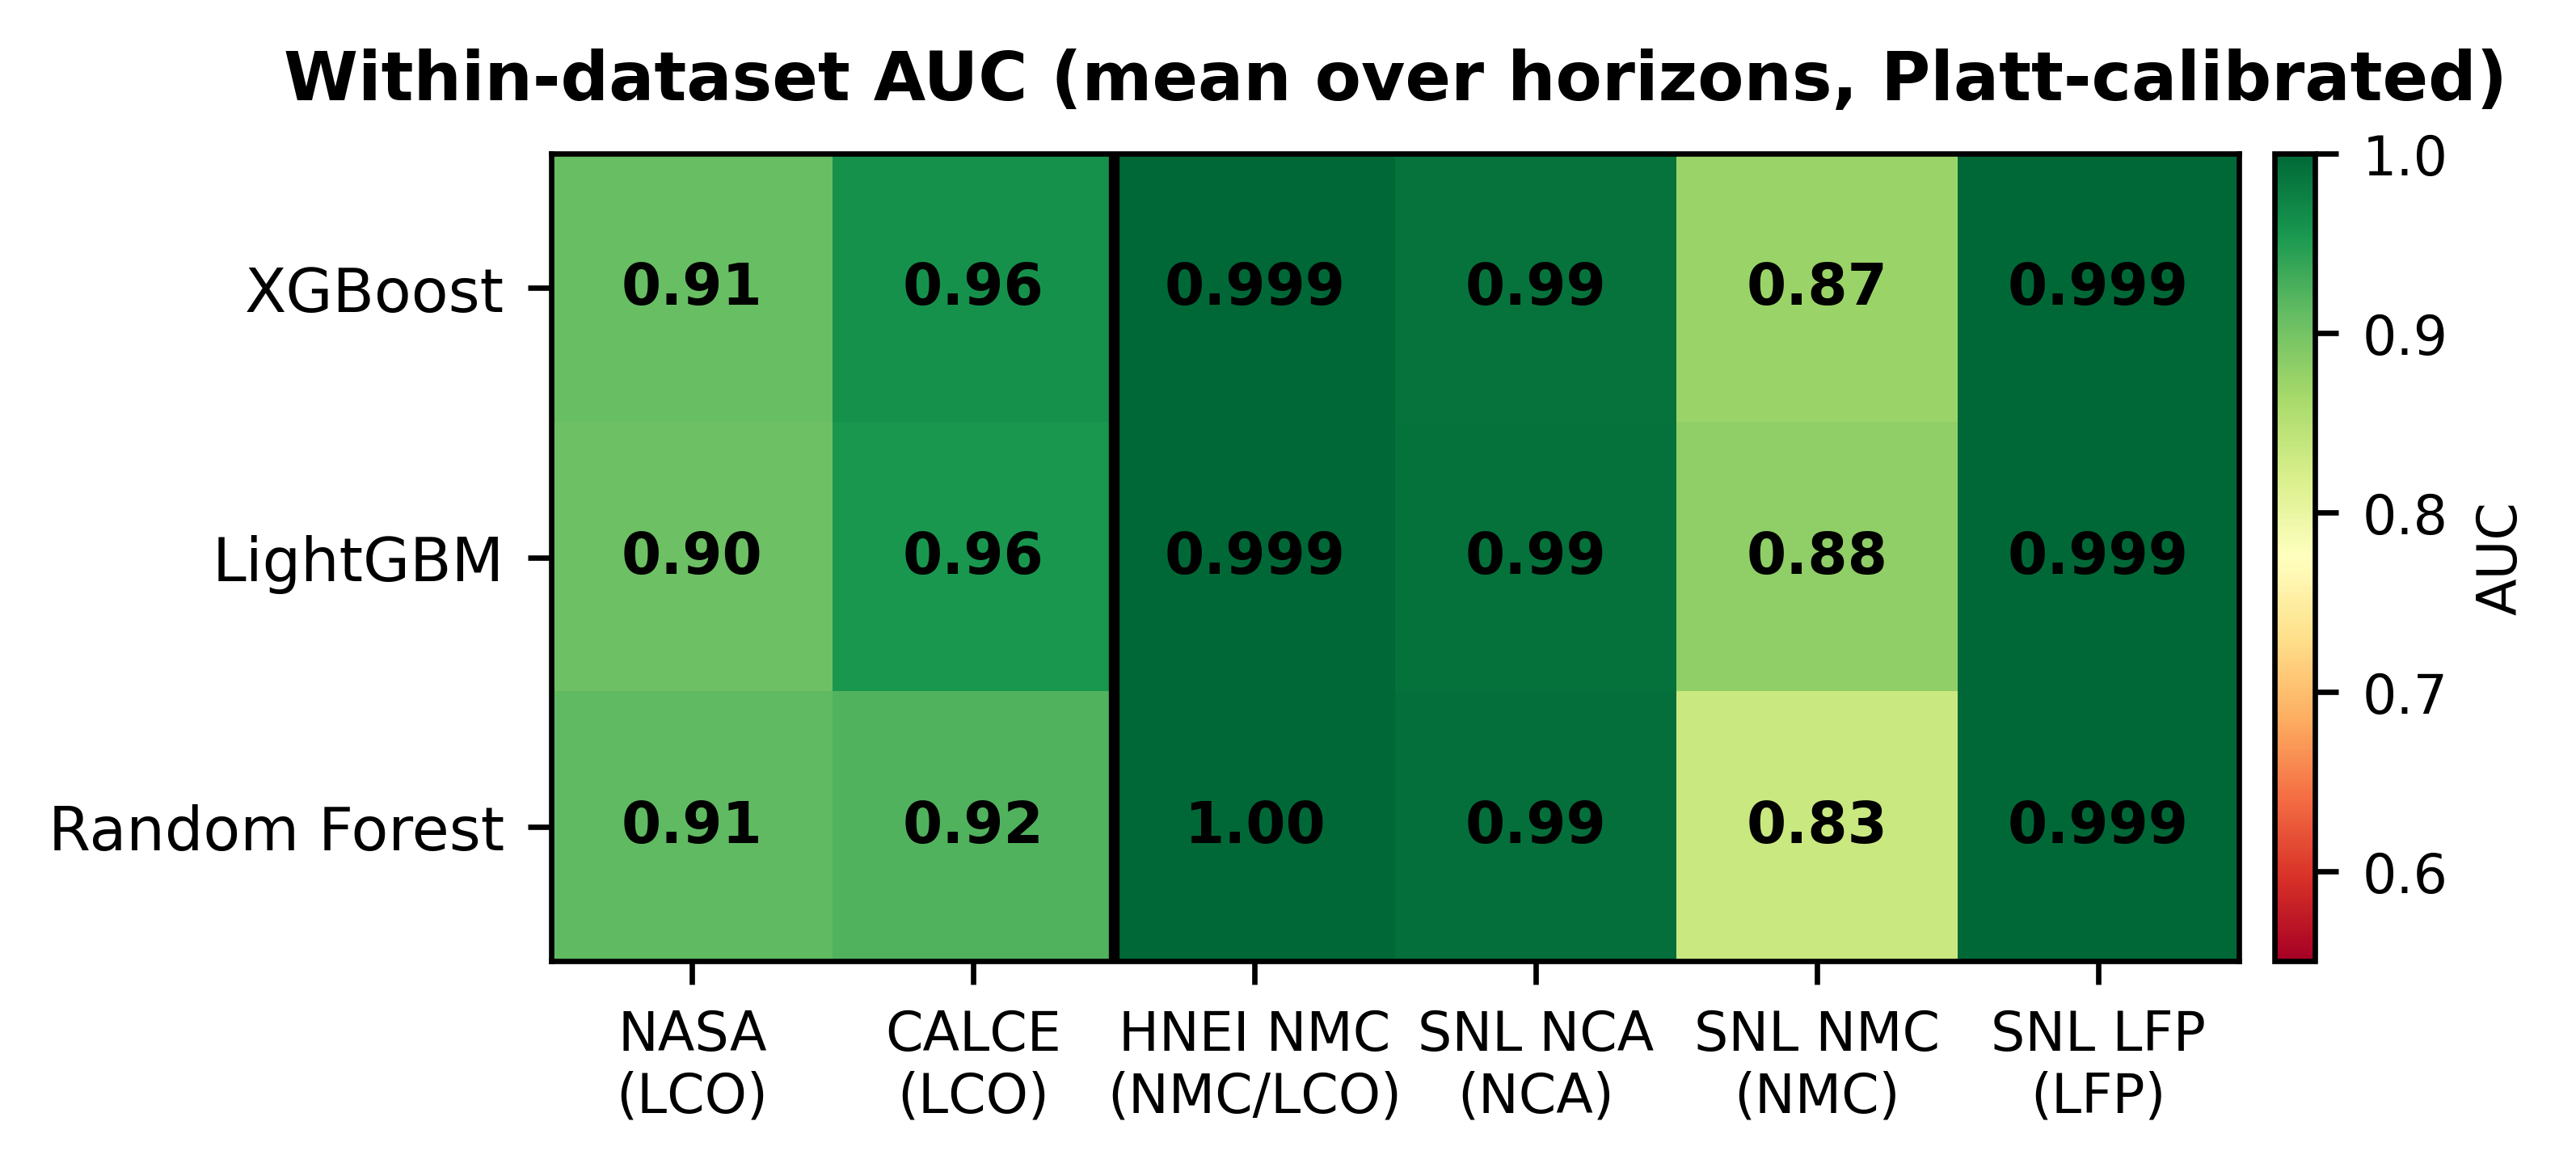
\includegraphics[width=0.78\textwidth]{Fig01_Within_Dataset_AUC.png}
\caption{Within-dataset AUC heatmap for the tree ensembles, mean across horizons, Platt-calibrated. Right block: the four new Battery Archive groups. GRU and hazard within-dataset numbers are in Table~\ref{tab:within}.}
\label{fig:within}
\end{figure}

\begin{figure}[!t]
\centering
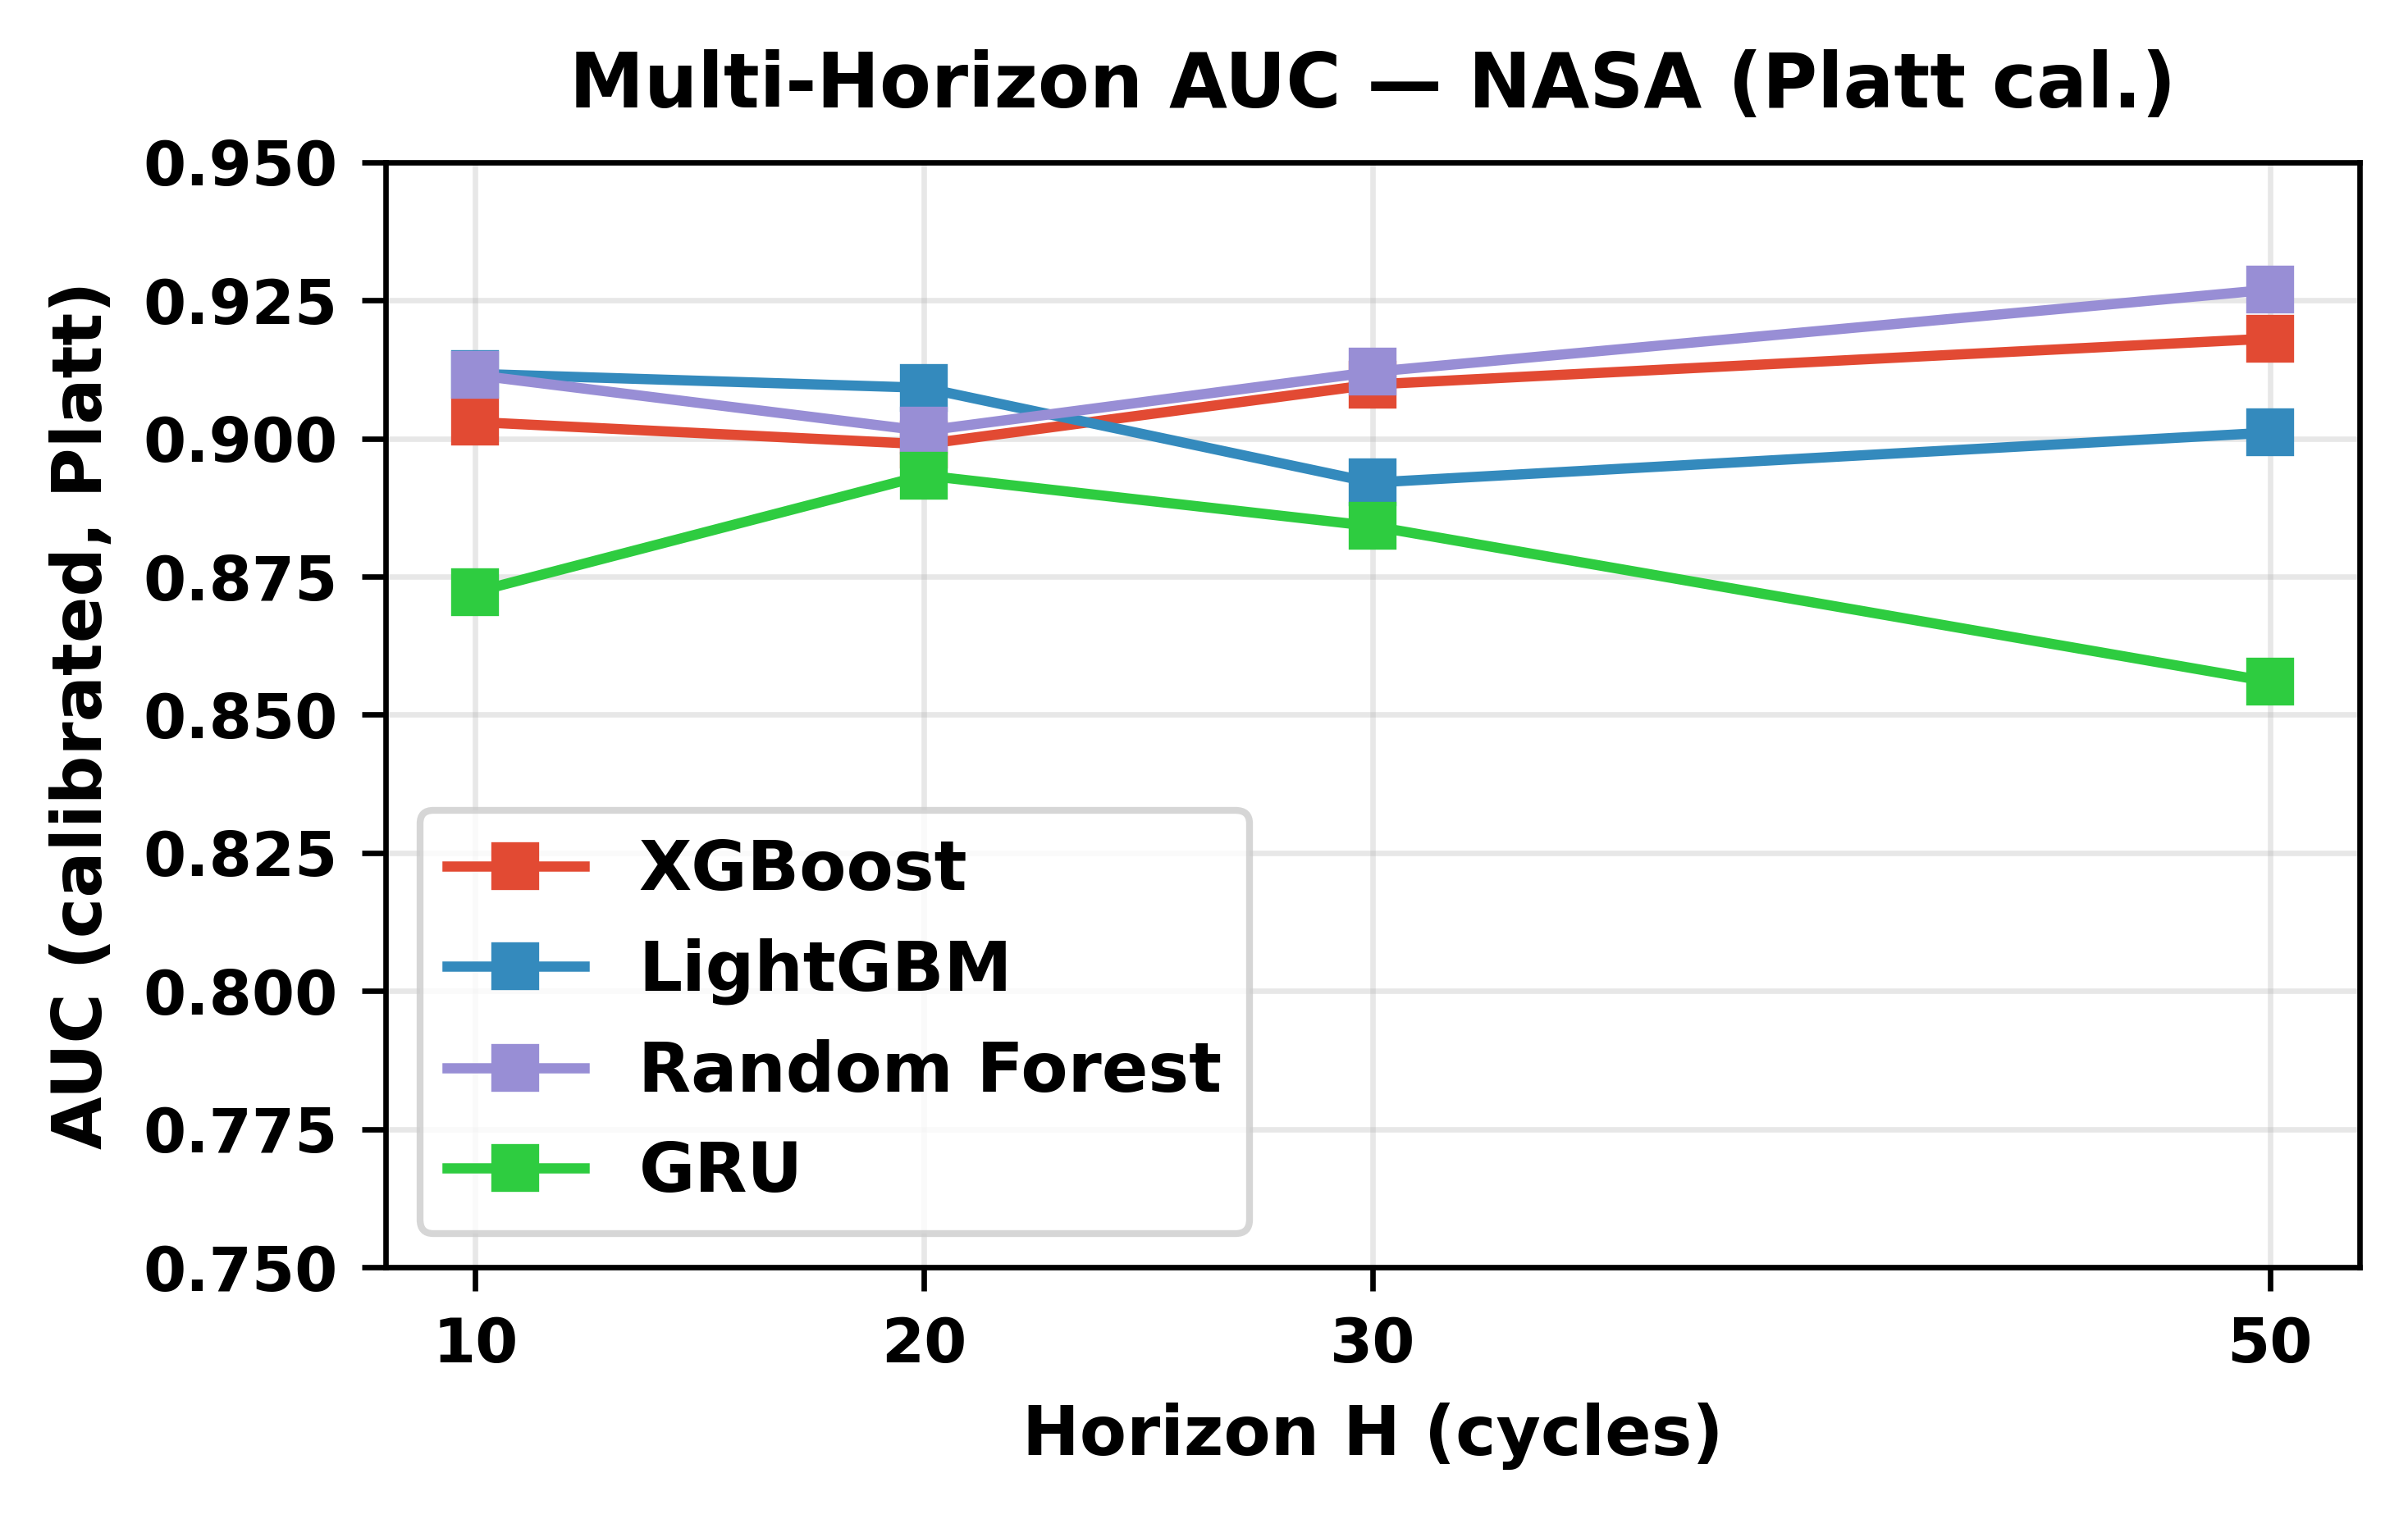
\includegraphics[width=0.78\textwidth]{Fig05_MultiHorizon_AUC.png}
\caption{Multi-horizon AUC on NASA at $H\in\{10,20,30,50\}$ (Platt-calibrated fold means). Values match Table~\ref{tab:within}.}
\label{fig:multihorizon}
\end{figure}

\subsection{Calibration Under Cross-Fitting}
Table~\ref{tab:cal} compares the three calibrators, averaged over the tree models and horizons, where every calibrator is fitted on cross-fitted out-of-fold scores. Three observations follow. First, on discrimination the raw scores are effectively unbeatable within dataset: any fitted calibrator is a monotone re-mapping and preserves per-fold ranking up to the ties it introduces, and the fold-mean AUC differences between calibrators are correspondingly small. Second, the step function of isotonic regression creates large tied groups whose cost is invisible to fold-mean ROC-AUC but severe for precision--recall: on NASA, raw scores reach a mean PR-AUC of 0.774 while isotonic collapses to 0.639 (Supplementary Material). Third, calibration quality proper is best for Platt on CALCE (ECE 0.029 against 0.049 for isotonic), but the fitted Platt slope on CALCE is only 0.011: in that long-tailed, leave-one-cell-out setting the out-of-fold sigmoid essentially washes confidence out toward the base rate while preserving ranking. Temperature scaling is the most balanced compromise on NASA (slope 1.218, Brier 0.178, both better than Platt's). There is no global winner across datasets, so we read the comparison as: \emph{Platt preserves discrimination best while achieving calibration error comparable to or better than isotonic} --- a materially weaker and more defensible claim than ``Platt is the better calibrator'' --- and raw scores remain the safest ranking signal whenever the operating context is uncertain.

\begin{table}[!t]
\caption{Calibration Quality Averaged Over Tree Models and Horizons. All Calibrators Are Fitted on Cross-Fitted Out-of-Fold Scores. Slope 1 / Intercept 0 Indicate Perfect Probabilistic Calibration.}
\label{tab:cal}
\centering
\scriptsize
\begin{tabular}{llcccccc}
\toprule
\textbf{Dataset} & \textbf{Method} & \textbf{AUC} & \textbf{Brier} & \textbf{ECE} & \textbf{Log loss} & \textbf{Slope} & \textbf{Int.}\\
\midrule
NASA & Isotonic & 0.854 & 0.207 & 0.151 & 0.652 & 0.48 & $-$0.26 \\
NASA & Platt & 0.908 & 0.196 & 0.136 & 0.575 & 0.90 & $-$0.14 \\

NASA & Temperature & 0.908 & 0.178 & 0.107 & 0.536 & 1.22 & $-$0.30 \\
CALCE & Isotonic & 0.915 & 0.067 & 0.049 & 0.279 & 0.41 & 1.17 \\
CALCE & Platt & 0.946 & 0.073 & 0.029 & 0.280 & 0.01 & 2.54 \\
CALCE & Temperature & 0.945 & 0.080 & 0.067 & 0.284 & 0.53 & 1.42 \\
\bottomrule
\end{tabular}
\end{table}

\subsection{Cross-Chemistry Transfer and the SOH Ablation}
Table~\ref{tab:crosswith} reports transfer from the LCO sources to the two LFP targets with SOH available, and Table~\ref{tab:crossno} repeats the identical protocol with SOH removed from the feature set (both at $H{=}20$; Figure~\ref{fig:collapse}). With SOH, transfer looks strong: pooled AUC spans 0.85--1.00 on Oxford and 0.85--0.90 on Severson, with per-cell means of 0.76--1.00. Removing SOH collapses every configuration toward or below chance: Oxford falls to 0.33--0.58 pooled AUC and Severson to 0.53--0.75. The paired cell-level bootstrap puts the with-minus-without difference on Severson at $+0.146$ [0.097, 0.233] for XGBoost at $H{=}20$, with positive intervals at every horizon for all three ensembles (deltas 0.10--0.18); Oxford point estimates agree ($+0.26$ to $+0.64$), but paired intervals are undefined with five cells, so Oxford contributes directional consistency only. On Severson the pooled numbers are dominated by long-lived cells; per-cell means without SOH remain as high as 0.88 (ALL-LCO Random Forest), so individual-cell ranking partially survives even where pooled transfer fails --- the two views bracket what actually transfers.

Three further observations tighten the attribution. First, the detection/prediction split of Section~2: because the labeling window includes the current cycle, with-SOH scores mix concurrent detection with future prediction. On Severson, 99.2\% of positive rows are scored before the failure crossing, and removing the remaining at-or-after-crossing rows drops with-SOH transfer from 0.896 to 0.838 [0.760, 0.991] and no-SOH transfer from 0.750 to 0.721 [0.666, 0.833] (ALL-LCO XGBoost); the unfitted distance rule drops from 0.912 to 0.862. With-SOH numbers are therefore diagnostic-proximity upper bounds rather than pure prognosis. Second, the compact GRU, evaluated on the common four-feature subset with three seeds, is not exempt: without SOH its per-cell transfer to Severson is 0.987$\pm$0.015 from the NASA source yet 0.479$\pm$0.451 from CALCE (individual seeds span 0.21--1.00) and 0.893$\pm$0.131 from ALL-LCO --- sequence representations can succeed where trees fail, but not reproducibly enough to carry a transfer claim. Third, calibration: isotonic maps fitted on source out-of-fold scores cost the tree ensembles up to 0.48 pooled AUC on Oxford and 0.31 on Severson under transfer even with SOH present, while Platt's smooth sigmoid degrades more gracefully (Section~3).

\begin{table}[!t]
\caption{Cross-Chemistry Transfer \textbf{With} SOH at $H{=}20$ (LCO Sources $\to$ LFP Targets): Pooled AUC [Cell-Level Bootstrap 95\% CI] and Per-Cell Mean $\pm$ SD.}
\label{tab:crosswith}
\centering
\footnotesize
\begin{tabular}{llcccc}
\toprule
 & & \multicolumn{2}{c}{\textbf{Oxford}} & \multicolumn{2}{c}{\textbf{Severson}}\\
\cmidrule(lr){3-4}\cmidrule(l){5-6}
\textbf{Training} & \textbf{Model} & \textbf{Pooled [CI]} & \textbf{Per-cell} & \textbf{Pooled [CI]} & \textbf{Per-cell}\\
\midrule
NASA & XGBoost & 0.957 [0.931,0.987] & 0.959$\pm$0.037 & 0.871 [0.767,0.997] & 0.997$\pm$0.010 \\
NASA & LightGBM & 1.000 [1.000,1.000] & 1.000$\pm$0.000 & 0.849 [0.724,0.998] & 0.992$\pm$0.048 \\
NASA & Random Forest & 1.000 [1.000,1.000] & 1.000$\pm$0.000 & 0.861 [0.739,0.998] & 0.999$\pm$0.007 \\
CALCE & XGBoost & 0.850 [0.764,0.910] & 0.763$\pm$0.245 & 0.850 [0.749,0.967] & 0.957$\pm$0.054 \\
CALCE & LightGBM & 0.889 [0.827,0.932] & 0.837$\pm$0.193 & 0.863 [0.782,0.957] & 0.952$\pm$0.037 \\
CALCE & Random Forest & 0.850 [0.773,0.899] & 0.766$\pm$0.169 & 0.902 [0.834,0.984] & 0.996$\pm$0.022 \\
ALL LCO & XGBoost & 0.917 [0.878,0.965] & 0.826$\pm$0.265 & 0.896 [0.812,0.995] & 0.995$\pm$0.015 \\
ALL LCO & LightGBM & 0.971 [0.959,0.981] & 0.969$\pm$0.015 & 0.882 [0.789,0.990] & 0.993$\pm$0.026 \\
ALL LCO & Random Forest & 0.989 [0.979,0.998] & 0.992$\pm$0.013 & 0.889 [0.796,0.998] & 0.996$\pm$0.021 \\
\bottomrule
\end{tabular}
\end{table}

\begin{table}[!t]
\caption{Cross-Chemistry Transfer \textbf{Without} SOH at $H{=}20$ (LCO Sources $\to$ LFP Targets): Same Protocol and Reporting as Table~\ref{tab:crosswith}.}
\label{tab:crossno}
\centering
\footnotesize
\begin{tabular}{llcccc}
\toprule
 & & \multicolumn{2}{c}{\textbf{Oxford}} & \multicolumn{2}{c}{\textbf{Severson}}\\
\cmidrule(lr){3-4}\cmidrule(l){5-6}
\textbf{Training} & \textbf{Model} & \textbf{Pooled [CI]} & \textbf{Per-cell} & \textbf{Pooled [CI]} & \textbf{Per-cell}\\
\midrule
NASA & XGBoost & 0.518 [0.513,0.522] & 0.519$\pm$0.006 & 0.595 [0.510,0.726] & 0.676$\pm$0.184 \\
NASA & LightGBM & 0.533 [0.497,0.543] & 0.448$\pm$0.201 & 0.527 [0.422,0.672] & 0.535$\pm$0.183 \\
NASA & Random Forest & 0.521 [0.487,0.537] & 0.442$\pm$0.198 & 0.674 [0.561,0.826] & 0.836$\pm$0.176 \\
CALCE & XGBoost & 0.416 [0.264,0.554] & 0.360$\pm$0.208 & 0.682 [0.670,0.695] & 0.806$\pm$0.082 \\
CALCE & LightGBM & 0.462 [0.307,0.579] & 0.410$\pm$0.207 & 0.643 [0.530,0.721] & 0.830$\pm$0.042 \\
CALCE & Random Forest & 0.501 [0.320,0.641] & 0.435$\pm$0.243 & 0.665 [0.547,0.749] & 0.870$\pm$0.049 \\
ALL LCO & XGBoost & 0.429 [0.279,0.597] & 0.415$\pm$0.240 & 0.750 [0.692,0.835] & 0.860$\pm$0.139 \\
ALL LCO & LightGBM & 0.332 [0.112,0.515] & 0.316$\pm$0.209 & 0.718 [0.634,0.850] & 0.808$\pm$0.167 \\
ALL LCO & Random Forest & 0.581 [0.516,0.644] & 0.608$\pm$0.103 & 0.746 [0.673,0.845] & 0.876$\pm$0.115 \\
\bottomrule
\end{tabular}
\end{table}

\begin{figure}[!t]
\centering
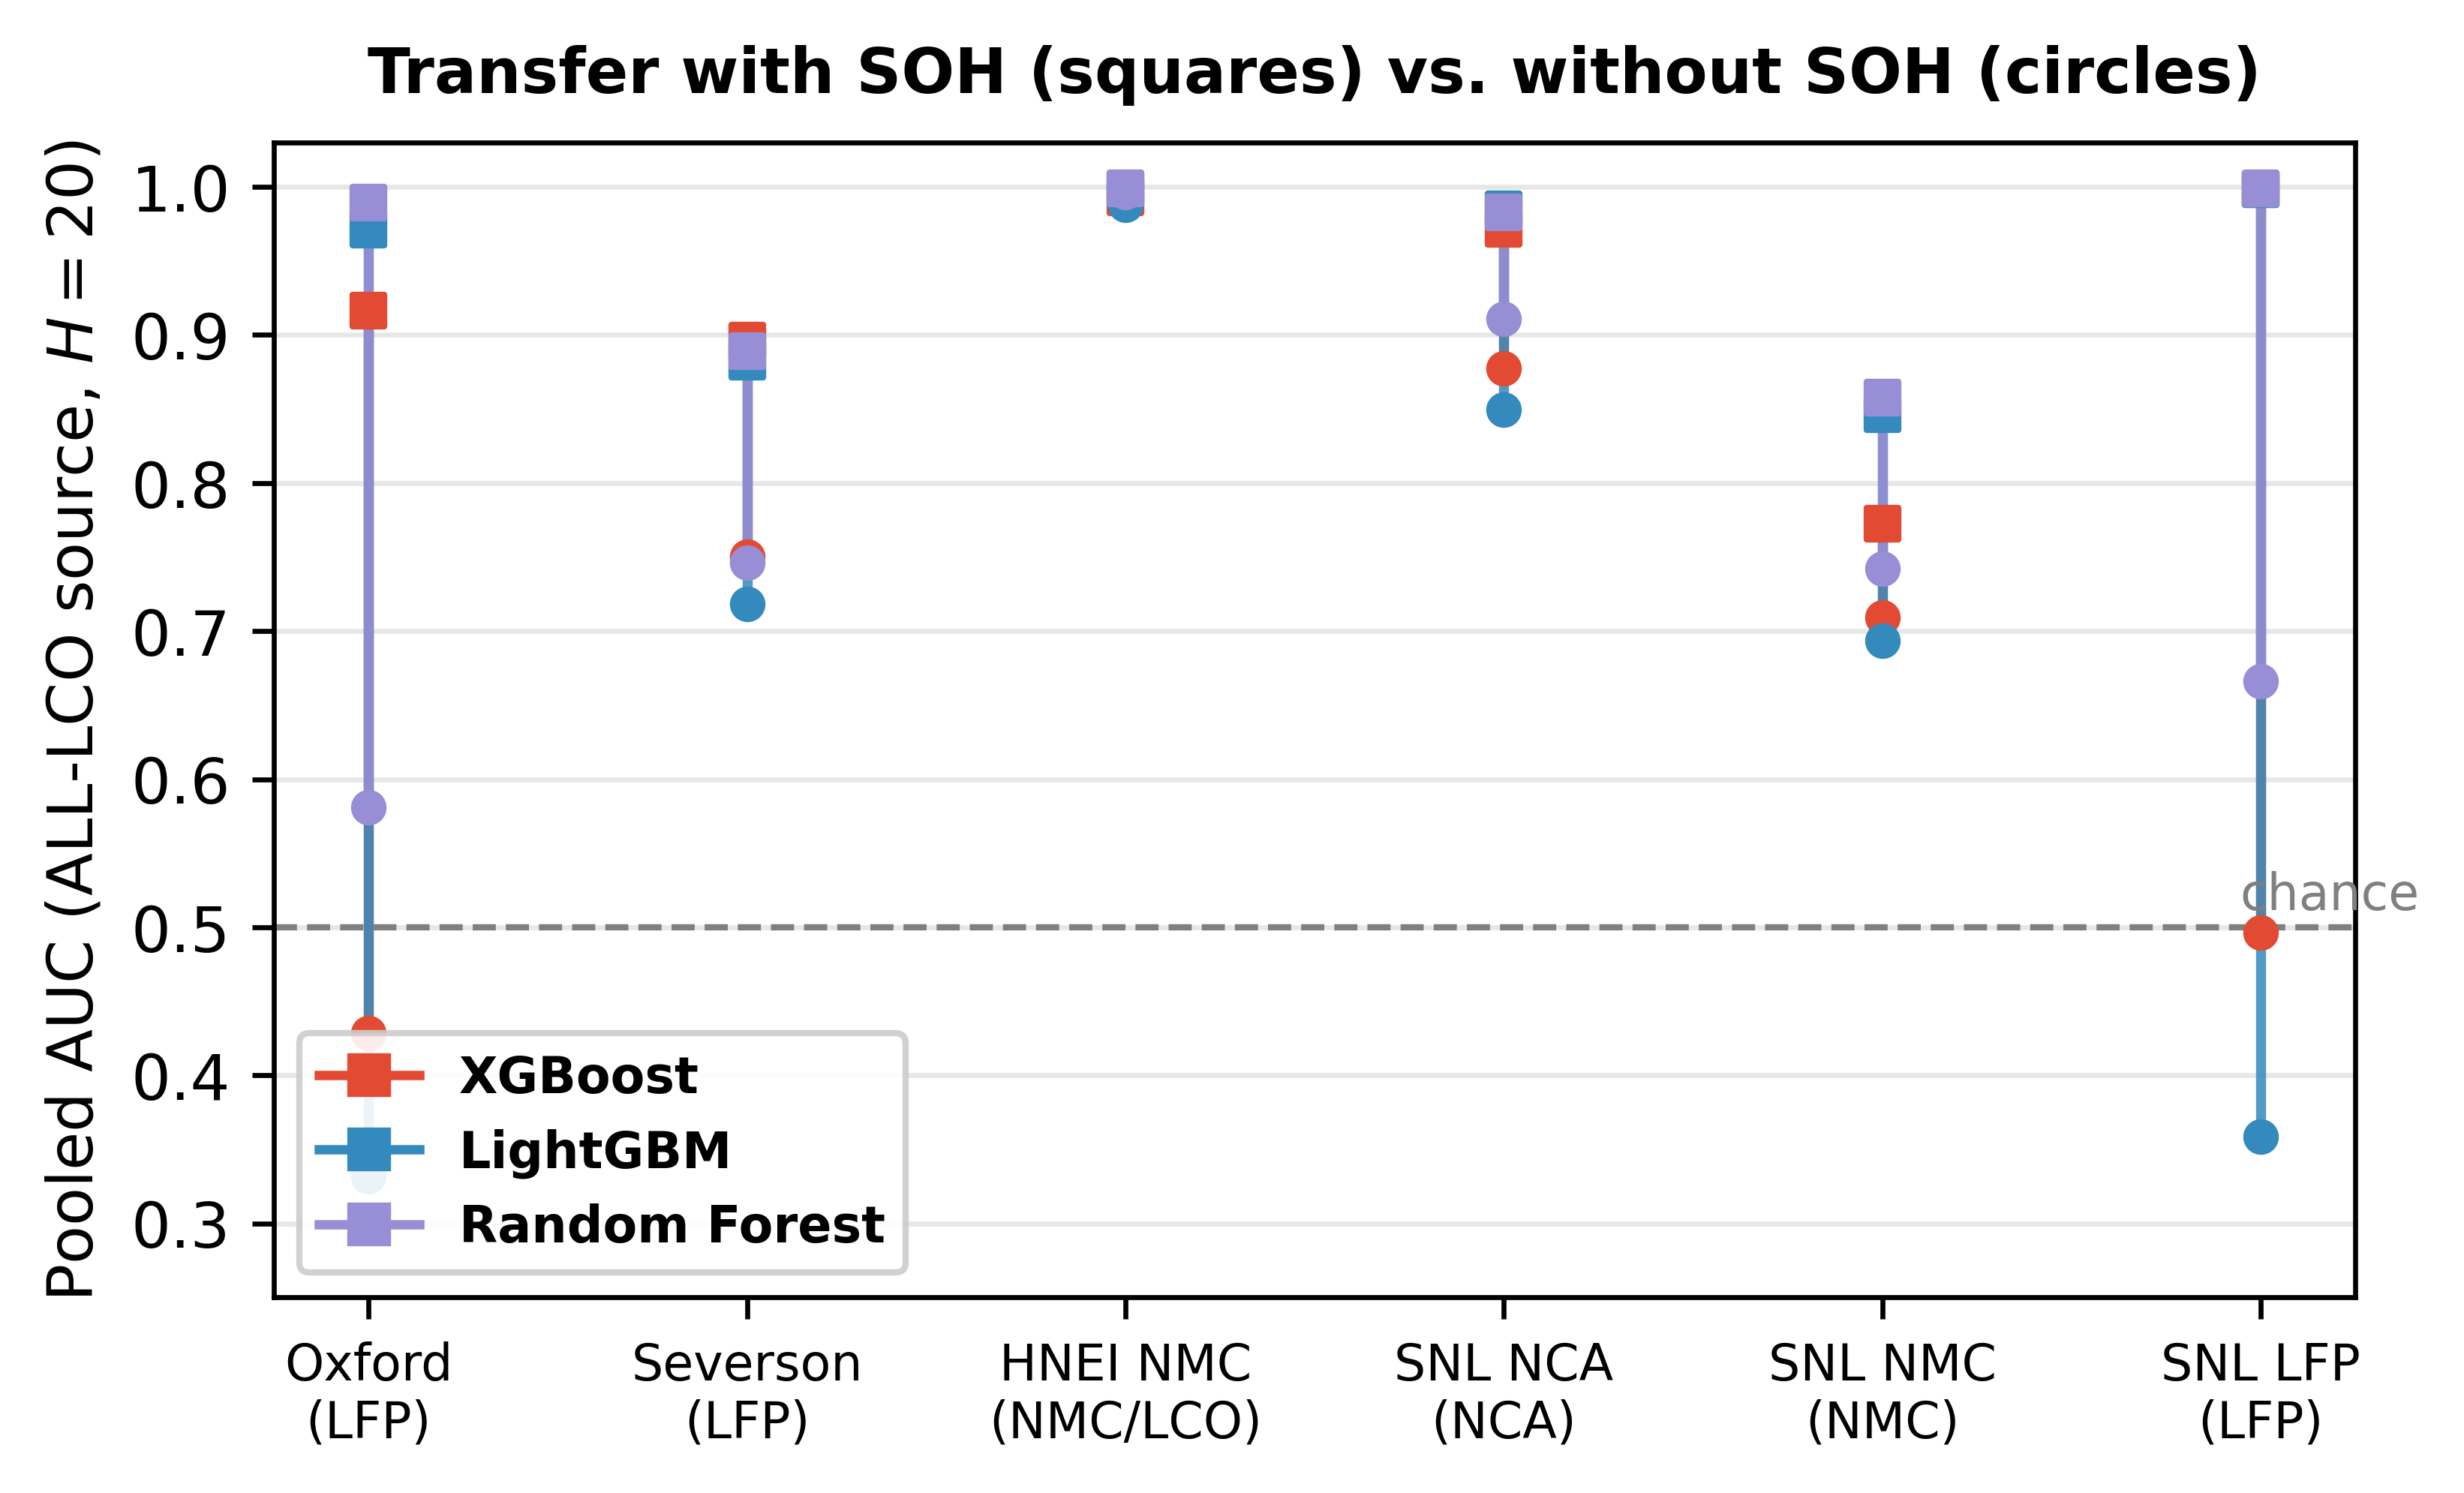
\includegraphics[width=0.78\textwidth]{Fig02_Transfer_Collapse.png}
\caption{Transfer from the ALL-LCO source at $H{=}20$ with SOH (squares) and without SOH (circles): pooled AUC per model on the two LFP targets and the four new Battery Archive groups. Removing SOH collapses every target except the single-condition HNEI group.}
\label{fig:collapse}
\end{figure}

\subsection{Minimal Baselines and the Factorial Feature Ablation}
Table~\ref{tab:baselines} places the tuned ensembles next to trivial baselines. The distance-to-threshold rule $d_t = 0.80 - \mathrm{SOH}_t$, which involves no fitting at all, transfers to Severson at pooled AUC 0.912 [0.836, 0.998] for every LCO source --- matching or exceeding the tuned ensembles' with-SOH transfer in Table~\ref{tab:crosswith}. An SOH-only logistic regression behaves equivalently (0.912). Both are diagnostic baselines by construction: they order cells by proximity to the label threshold, not by learned degradation dynamics. By contrast, the sensor-only logistic regression transfers at 0.301 on Severson (NASA source): below chance, meaning the remaining sensor features actively invert on the shifted distribution. Within CALCE, the cycle index alone ranks failure at pooled AUC 0.936, approaching the tuned ensembles, because CALCE's seven cells span very different cycle lives; on NASA, whose cells age under randomized profiles, the same feature is inverted (0.354).

The full $2^3-1$ factorial grid over \{SOH, cycle index, sensors\} at $H{=}20$ sharpens the diagnosis (Supplementary Material). SOH-only is the strongest single group on both LFP targets, confirming that the health coordinate dominates whatever transfer exists. Cycle-only is competitive on Oxford in the logistic baselines (0.99, NASA source) --- whose five cells fail at well-separated raw cycle counts, so the cycle index is a between-cell aging proxy --- but not in the factorial XGBoost grid itself (0.54 on Oxford, 0.71 on Severson): the pattern is model- and source-specific, not portable degradation knowledge. No combination without SOH reaches 0.76 on either target (best 0.75), and removing both SOH and the cycle index leaves the sensors with essentially nothing (0.535 with the ALL-LCO source on Severson). The ablation makes the shortcut diagnosis feature-by-feature: it is not that the models fail to use the sensor features; it is that the sensor features themselves carry no cross-dataset signal.

Three conclusions follow. First, most of what transfers is the SOH coordinate, not degradation knowledge. Second, ``more features'' does not help transfer; sensor features carry dataset-specific artifacts that can invert. Third, the ensembles' within-dataset value is undiminished --- but the transfer claim must be downgraded from ``models transfer'' to ``the health state transfers, and models can read it.''

\begin{table}[!t]
\caption{Minimal Transfer Baselines at $H{=}20$: Pooled AUC With Cell-Level Bootstrap 95\% CI. The Distance Rule Is the Unfitted Score $0.80-$SOH.}
\label{tab:baselines}
\centering
\footnotesize
\setlength{\tabcolsep}{3pt}
\begin{tabular}{>{\raggedright\arraybackslash}p{2.0cm}*{6}{>{\raggedright\arraybackslash}p{2.05cm}}}
\toprule
 & \multicolumn{3}{c}{\textbf{Oxford}} & \multicolumn{3}{c}{\textbf{Severson}}\\
\cmidrule(lr){2-4}\cmidrule(l){5-7}
\textbf{Baseline} & \textbf{NASA src} & \textbf{CALCE src} & \textbf{ALL src} & \textbf{NASA src} & \textbf{CALCE src} & \textbf{ALL src}\\
\midrule
SOH distance rule & 1.000 [1.000,1.000] & 1.000 [1.000,1.000] & 1.000 [1.000,1.000] & 0.912 [0.836,0.998] & 0.912 [0.836,0.998] & 0.912 [0.836,0.998] \\
SOH only & 1.000 [1.000,1.000] & 1.000 [1.000,1.000] & 1.000 [1.000,1.000] & 0.912 [0.836,0.998] & 0.912 [0.836,0.998] & 0.912 [0.836,0.998] \\
cycle only & 0.989 [0.983,1.000] & 0.756 [0.732,0.780] & 0.787 [0.760,0.814] & 0.713 [0.591,0.798] & 0.713 [0.591,0.798] & 0.713 [0.591,0.798] \\
SOH + cycle & 0.990 [0.985,1.000] & 0.797 [0.770,0.825] & 0.818 [0.788,0.848] & 0.865 [0.834,0.902] & 0.764 [0.674,0.829] & 0.758 [0.664,0.825] \\
sensors only & 0.500 [0.500,0.500] & 0.500 [0.500,0.500] & 0.500 [0.500,0.500] & 0.301 [0.015,0.549] & 0.498 [0.497,0.500] & 0.303 [0.059,0.497] \\
full (7 feats) & 0.500 [0.500,0.500] & 0.500 [0.500,0.500] & 0.500 [0.500,0.500] & 0.823 [0.675,0.995] & 0.712 [0.589,0.797] & 0.674 [0.525,0.782] \\
\bottomrule
\end{tabular}
\end{table}

\subsection{Failure-Definition Ablation: Measuring the Label Circularity}
Table~\ref{tab:faildef} relabels failure by a single endpoint at a time and repeats the transfer experiments. This quantifies the circularity concern of Section~2: with-SOH transfer \emph{tracks how much SOH defines the label}. Under the SOH-only label, transfer to Severson is 0.985; under the combined label, 0.896. Relabel by voltage sag alone and with-SOH transfer falls to 0.723 --- a drop of about 0.17, with the with-minus-without gap narrowing from $+0.15$ to $+0.11$. The residual (0.723 versus 0.611) is genuine but weak health-state information. Within one laboratory the distinction nearly vanishes --- on NASA the with-SOH model reaches 0.936 under the SOH-only endpoint (0.760 under the combined endpoint) --- because sensor features co-move with SOH there; dataset shift destroys that co-movement, and with it the transfer illusion.

\begin{table}[!t]
\caption{Failure-Definition Ablation at $H{=}20$ (XGBoost, ALL-LCO Source, Pooled AUC [CI]): Transfer With and Without SOH as a Feature, for Three Label Endpoints.}
\label{tab:faildef}
\centering
\footnotesize
\begin{tabular}{lcccc}
\toprule
 & \multicolumn{2}{c}{\textbf{Oxford}} & \multicolumn{2}{c}{\textbf{Severson}}\\
\cmidrule(lr){2-3}\cmidrule(l){4-5}
\textbf{Label endpoint} & \textbf{with SOH} & \textbf{no SOH} & \textbf{with SOH} & \textbf{no SOH}\\
\midrule
Combined (SOH or sag) & 0.917 [0.878,0.965] & 0.429 [0.279,0.597] & 0.896 [0.812,0.995] & 0.750 [0.692,0.835] \\
SOH only & 0.995 [0.988,1.000] & 0.464 [0.320,0.596] & 0.985 [0.977,0.992] & 0.759 [0.709,0.801] \\
Voltage sag only & --- & --- & 0.723 [0.705,0.740] & 0.611 [0.585,0.637] \\
\bottomrule
\end{tabular}
\end{table}

\subsection{Same-Chemistry Cross-Laboratory Controls}
If the collapse of Section~3 were a chemistry effect, transfer should survive when chemistry is held constant. Table~\ref{tab:samechem} shows it does not. NASA$\to$CALCE (both LCO) retains most of its transfer without SOH, so some laboratory pairs do share portable sensor signal; but Severson$\to$Oxford (both LFP) reproduces the full collapse pattern of the cross-chemistry shifts, including high with-SOH transfer and near-chance sensor-only transfer. These controls tighten the central attribution: the failure to transfer is a property of \emph{dataset shift} --- laboratories, protocols, and logging conventions --- that chemistry change adds to but does not uniquely cause. SOH is therefore a \emph{dataset- and chemistry-dependent} health-state signal, not a chemistry-specific one, and chemistry is not isolated as a causal variable.

\begin{table}[!t]
\caption{Same-Chemistry Cross-Laboratory Controls at $H{=}20$ (XGBoost, Pooled AUC [CI]). Full Feature Sets Exercise the Zero-Imputation Confound; Common Sets Restrict Both Datasets to the Shared Four-Feature Subset.}
\label{tab:samechem}
\centering
\footnotesize
\begin{tabular}{lccc}
\toprule
\textbf{Pair} & \textbf{with SOH (full)} & \textbf{no SOH (full)} & \textbf{no SOH (common)}\\
\midrule
NASA$\to$CALCE (LCO$\to$LCO) & 0.870 [0.799,0.966] & 0.849 [0.753,0.985] & 0.781 [0.708,0.964] \\
CALCE$\to$NASA (LCO$\to$LCO) & 0.543 [0.356,0.677] & 0.566 [0.427,0.678] & 0.601 [0.496,0.703] \\
Severson$\to$Oxford (LFP$\to$LFP) & 0.997 [0.991,1.000] & 0.471 [0.466,0.477] & 0.428 [0.422,0.435] \\
Oxford$\to$Severson (LFP$\to$LFP) & 0.688 [0.605,0.788] & 0.500 [0.500,0.500] & 0.500 [0.500,0.500] \\
\bottomrule
\end{tabular}
\end{table}

\subsection{Discrete-Time Hazard Model and Monotonicity}
Within datasets the survival product of Section~2 matches the independent fixed-horizon classifiers to within a few AUC points at every horizon (Table~\ref{tab:within}); no formal equivalence test is run. Under transfer the survival product inherits the same SOH dependence --- the ALL-LCO hazard XGBoost transfers to Oxford at pooled AUC 0.314, significantly below chance, and the hazard logistic degenerates to exactly 0.500 on three of six source--target pairs --- so model formulation does not exempt inputs from dataset shift. What the hazard formulation buys is structural: $R(t,H)$ is monotone in $H$ by construction, whereas the four independent classifiers violate $p_{10}\le p_{20}\le p_{30}\le p_{50}$ on 32--45\% of within-dataset rows (raw scores; 5.6--26\% after Platt calibration), rising to 95.8\% on transferred Severson rows (NASA-trained XGBoost). Monotone cumulative risk is what makes ``risk within 50 cycles'' coherent to quote: the hazard model buys structural coherence and a single fit at no within-dataset cost, and pays the same SOH shortcut as every other model. The full monotonicity table is in the Supplementary Material.

\subsection{Calibration Transfer and Its Partial Repair}
A second, independent failure mode appears when calibrated outputs are required under transfer. Isotonic regression is fitted as a step function on the source distribution; when target scores shift, many target scores fall into one bin and receive identical calibrated probabilities, and pooled ranking degrades accordingly --- isotonic calibration costs the tree ensembles up to 0.48 pooled AUC on Oxford and 0.31 on Severson even with SOH present (Section~3). Platt's smooth sigmoid degrades more gracefully, which is precisely the sense in which Platt better preserves discrimination at comparable calibration error (Section~3). On the shifted target, no source-fitted calibrator lands near the diagonal, however it is fitted.

A final experiment asks whether a small labeled target sample repairs this. In Arm~A a calibrator is refitted on $k$ labeled target cells while the classifier's scores are left untouched; in Arm~B the classifier continues training on them. On Severson without SOH, zero-shot ECE is 0.817; at $k{=}5$ labeled cells, isotonic and Platt reduce it to 0.044 and 0.045, while temperature scaling remains poorly calibrated (0.563). Calibration error is repaired, but discrimination is not: mean pooled AUC at $k{=}5$ stays near 0.61, because the calibrators create ties or reverse rankings on the shifted target. Arm~B is source-dependent: with NASA-trained XGBoost and $k{=}5$, Severson AUC rises from 0.620 to 0.854, overshooting the within-LCO reference ceiling (ratio 1.04, an artifact of the mismatched ceiling rather than genuine super-ceiling recovery), while CALCE-trained updates leave the source operating point essentially untouched (LCO-holdout retention 0.997 to 0.996) and ALL-LCO updates damage it substantially (0.690 to 0.567). Both arms are tabulated in the Supplementary Material.

\subsection{Operational Cost Analysis}
AUC treats all errors as equal; a BMS does not. We select the threshold on source out-of-fold scores with a 10\% false-alarm budget and apply it unchanged to the target (Table~\ref{tab:oper}). On Severson with SOH, the transferred XGBoost threshold misses 32\% of failures at 4\% false alarms. The same protocol fails for the other ensembles with SOH: LightGBM alerts on 65\% of negatives and Random Forest misses 100\% of failures --- threshold transfer fails for two of three ensembles even where ranking transfers. Without SOH, the XGBoost miss rate more than doubles to 70\% at 10\% false alarms; calibrated score types do not differ, because under shift the ranking is the asset and the ranking collapsed. On Oxford, nearly every row is positive, so no discriminating operating point exists there at all. The decision-curve view agrees: with SOH the model buys net benefit across thresholds; without SOH the curve hugs zero.

\begin{table}[!t]
\caption{Operational Evaluation at $H{=}20$ (XGBoost, ALL-LCO Source): Decision Threshold Selected on Source Out-of-Fold Scores With a 10\% False-Alarm Budget, Then Applied Unchanged to the Target. Reported Are the Target Miss Rate (FNR) and Target False-Alarm Rate (FPR).}
\label{tab:oper}
\centering
\scriptsize
\setlength{\tabcolsep}{2.5pt}
\begin{tabular}{llcccccccc}
\toprule
 & & \multicolumn{2}{c}{\textbf{raw}} & \multicolumn{2}{c}{\textbf{Platt}} & \multicolumn{2}{c}{\textbf{isotonic}} & \multicolumn{2}{c}{\textbf{temperature}}\\
\cmidrule(lr){3-4}\cmidrule(l){5-6}\cmidrule(l){7-8}\cmidrule(l){9-10}
\textbf{Target} & \textbf{Features} & \textbf{FNR} & \textbf{FPR} & \textbf{FNR} & \textbf{FPR} & \textbf{FNR} & \textbf{FPR} & \textbf{FNR} & \textbf{FPR}\\
\midrule
Oxford & with SOH & 0\% & 93\% & 0\% & 93\% & 0\% & 93\% & 0\% & 93\% \\
Oxford & no SOH & 0\% & 92\% & 0\% & 92\% & 0\% & 92\% & 0\% & 92\% \\
Severson & with SOH & 32\% & 4\% & 32\% & 4\% & 31\% & 6\% & 32\% & 4\% \\
Severson & no SOH & 70\% & 10\% & 70\% & 10\% & 67\% & 12\% & 70\% & 10\% \\
\bottomrule
\end{tabular}
\end{table}

\subsection{SHAP Attribution}
TreeSHAP \cite{lundberg2020from} gives a direct view of the mechanism. Attributions for the three tree models in NASA$\to$Oxford transfer at $H{=}20$ with SOH kept show SOH dominating by a wide margin, the cycle index a distant second, and the voltage, current, temperature, and duration features contributing little; with SOH removed, every remaining feature collapses to near-zero attribution spread --- matching, in the model's internal accounting, the quantitative collapse of Sections~3.3--3.5 and the sensor inversion of Section~3.

\subsection{Embedded Deployment Validation}
Three independent validation stages confirm that the C tree engine of Section~2 reproduces the Python training libraries through the output transforms of \eqref{eq:rf} and \eqref{eq:sigmoid}: a Python walker over the extracted trees, the same walker cross-compiled as an x86\_64 binary, and on-target execution on an ESP32-S3 against the library's \texttt{predict\_proba()} --- all below the $10^{-5}$ acceptance tolerance. On-device, the measured maximum absolute error over all 1~028 NASA rows is $2.4\times10^{-7}$ for XGBoost, $1.1\times10^{-6}$ for LightGBM, and $3.0\times10^{-8}$ for Random Forest.

Table~\ref{tab:deploy} lists sizes, validation error, and inference time; Figure~\ref{fig:deploy} plots latency and footprint. The ensembles occupy about 372 kB. At 240 MHz: from flash, 0.76, 1.55, and 2.36 ms per model; from PSRAM, 0.50, 0.93, and 1.29 ms; single-model from internal SRAM, 0.32, 0.43, and 0.50 ms. The full 372 kB binary does not fit internal SRAM (free heap roughly 320 kB), but each model does, and the firmware runs one model at a time. Timings land above the 150--250 \textmu s projection because the working set exceeds the ESP32-S3's data cache; even so, the all-three PSRAM path clears the 100 ms per-cycle budget by roughly 37\texttimes. The deployment result is deliberately independent of the validity question: whatever the models are reading, on this dataset they can read it in under a millisecond on a \$12 microcontroller. The on-device outputs are raw ensemble probabilities through \eqref{eq:rf}--\eqref{eq:sigmoid} with no calibration layer: the Platt and isotonic maps live off-device, and Section~3 shows source-fitted maps do not survive dataset shift, so a deployed system must revalidate or refit its calibrator on target-labeled cells rather than trust the laboratory calibration.

\begin{table}[!t]
\caption{Embedded Deployment: Model Size, On-Device Validation Error, and Measured Inference Time. Errors Are Maximum $|$C engine $-$ \texttt{predict\_proba()}$|$ Over All 1~028 Rows. Timings Measured On-Device at 240 MHz With the Binary in Flash (PROGMEM), PSRAM, or a Single Model in Internal SRAM.}
\label{tab:deploy}
\centering
\footnotesize
\setlength{\tabcolsep}{4pt}
\begin{tabular}{lrcccc}
\toprule
\textbf{Model} & \textbf{Nodes} & \textbf{Max Err} & \textbf{Flash} & \textbf{PSRAM} & \textbf{SRAM}\\
\midrule
XGBoost & 3\,272 & $2.4\times10^{-7}$ & 0.76 ms & 0.50 ms & 0.32 ms\\
LightGBM & 7\,000 & $1.1\times10^{-6}$ & 1.55 ms & 0.93 ms & 0.43 ms\\
Random Forest & 16\,064 & $3.0\times10^{-8}$ & 2.36 ms & 1.29 ms & 0.50 ms\\
All three & 26\,336 & --- & 4.7 ms & 2.7 ms & ---\\
\bottomrule
\end{tabular}
\end{table}

\begin{figure}[!t]
\centering
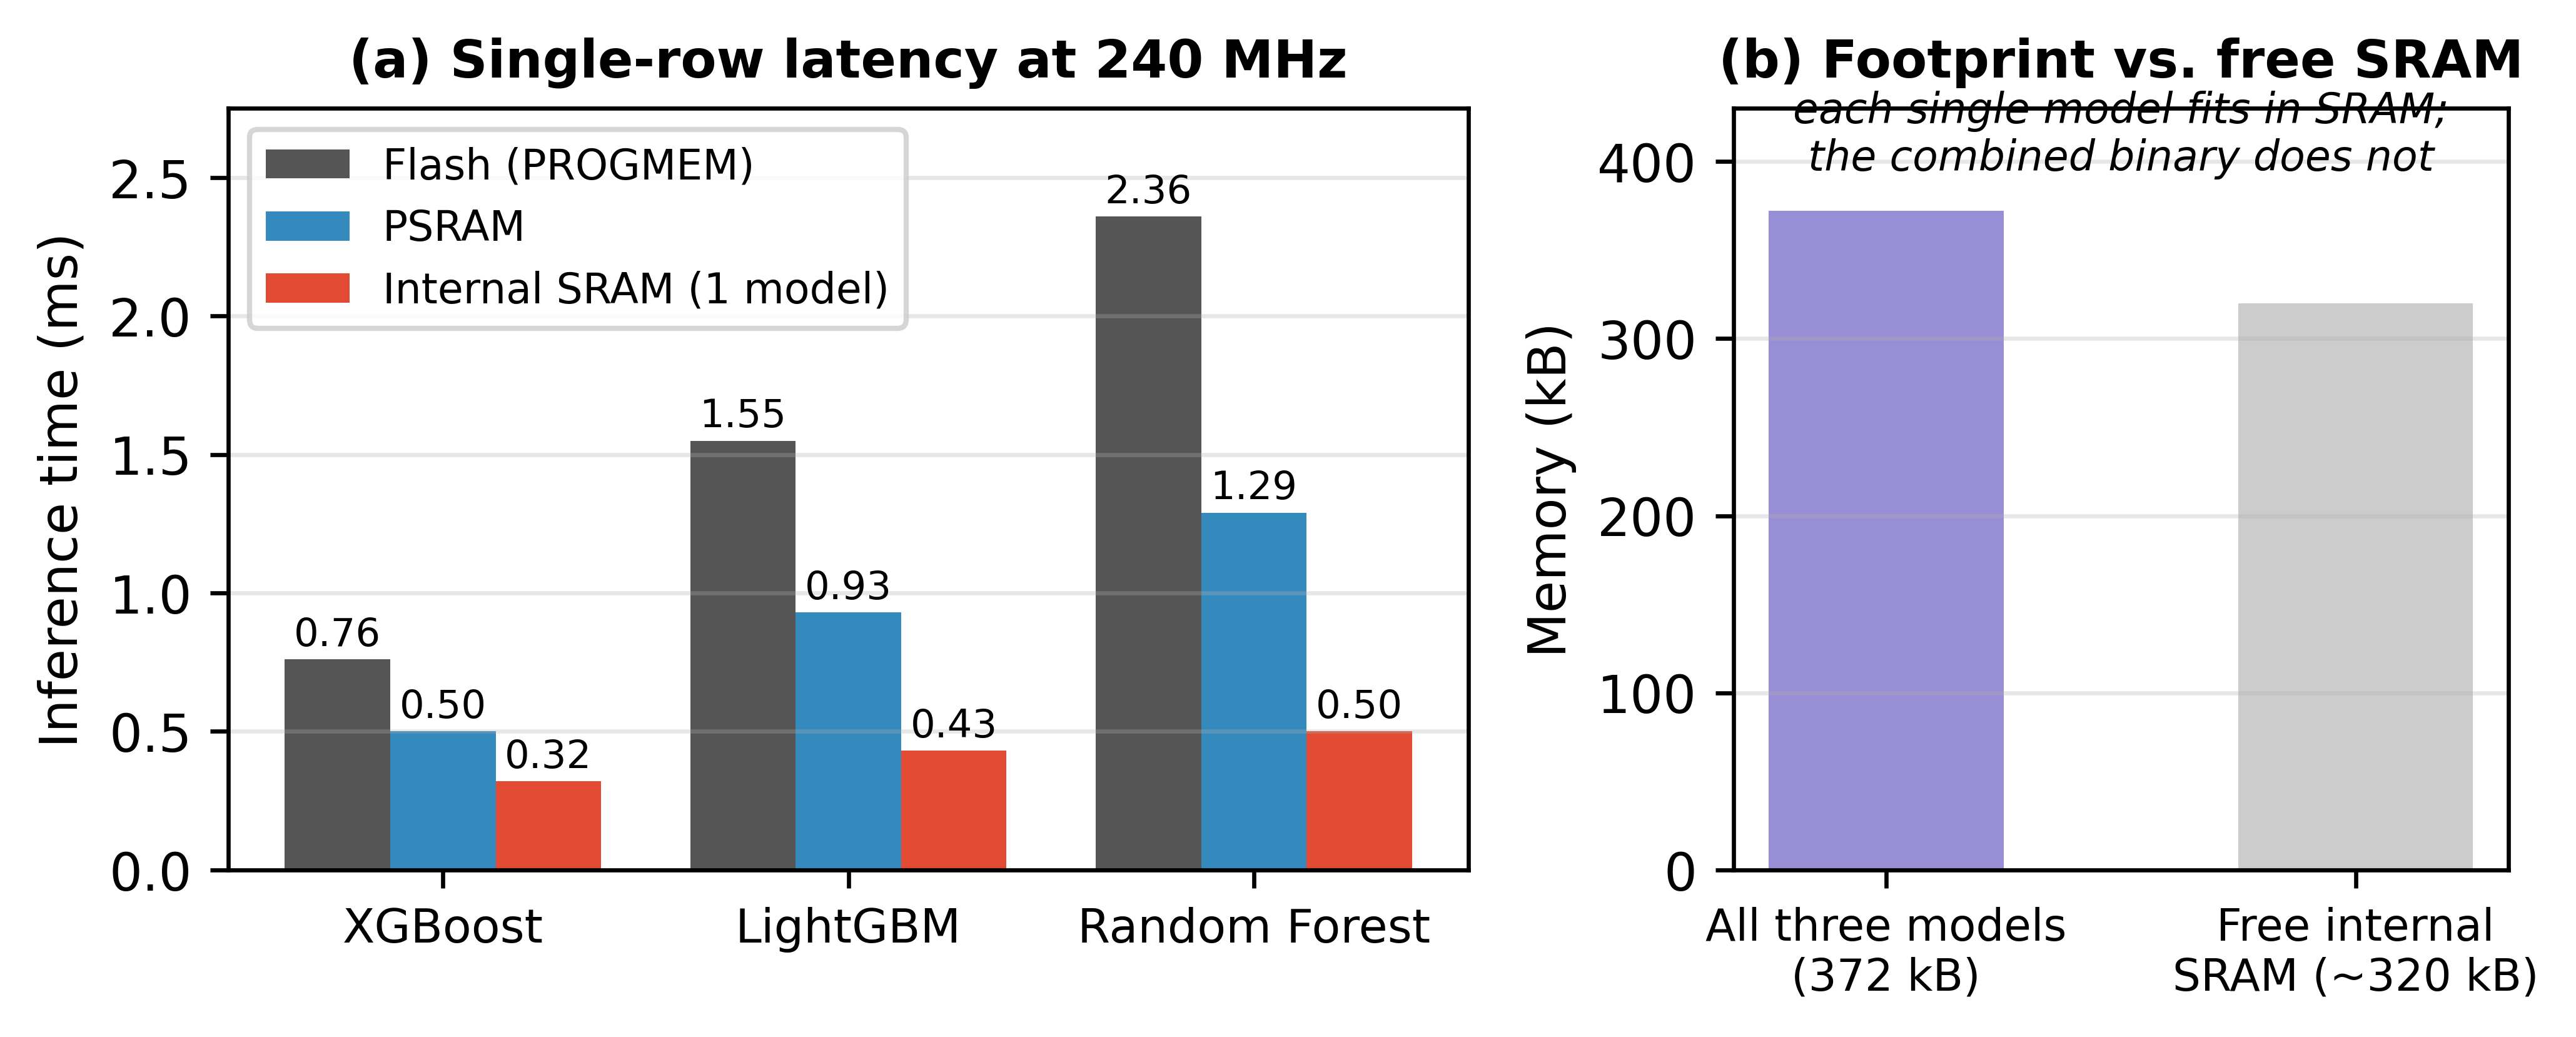
\includegraphics[width=0.78\textwidth]{fig_deploy.png}
\caption{Deployment trade-offs: (a) measured single-row inference time per model at 240 MHz with the binary in memory-mapped flash, PSRAM, or a single model in internal SRAM; (b) the combined 372 kB binary against the ESP32-S3's roughly 320 kB of free internal SRAM --- each model fits, the combined binary does not.}
\label{fig:deploy}
\end{figure}

\subsection{Replication on New Chemistries: NCA, NMC, and LFP Transfer Targets}
The transfer claim is re-tested on 60 cells of NMC, NCA and LFP chemistry from two further laboratories (Battery Archive groups 5--8 of Section~2), with the LCO training pool and protocol untouched --- the new cells never enter model selection --- and the experiment run on the same protocol version as every result above. Of 75 downloaded cells, 60 pass the pre-registered cleaning rule of Section~2 and 15 are excluded, all 15 for mixed state-of-charge windows. Table~\ref{tab:crosschemnew} reports the NASA+CALCE $\rightarrow$ new-target transfer at $H{=}20$, with and without SOH, together with the paired cell-level bootstrap for the SOH ablation.

With SOH available, transfer from the LCO sources spans pooled AUC 0.77--1.00 across the new targets --- the same upper-bound regime as Table~\ref{tab:crosswith}. Removing SOH drops transfer to 0.36--1.00, and the paired per-cell bootstrap puts the with-minus-without difference at 0.00--0.64 AUC across the three ensembles --- on the SNL groups the LCO-trained ensemble contributes nothing portable on NCA, NMC, or LFP chemistry from an unseen laboratory, exactly as it contributed nothing on the earlier LFP targets. The HNEI NMC group is the exception: full no-SOH transfer (cycle index included) stays at 0.99 pooled there. All 15 HNEI cells cycle under one condition and one fixed charge protocol, so cycle-index and voltage cues survive the laboratory change; this is the dataset-shift mechanism of Section~3 operating in reverse --- narrow, stereotyped protocols transfer, diverse ones do not --- not chemistry-specific knowledge. On the new groups the voltage-sag endpoint never fires before the SOH endpoint (0 of 60 admitted cells), so the composite label is, effectively, the SOH criterion alone; the failure-definition ablation of Section~3 therefore cannot be re-run on these targets, and all with-SOH numbers here are to be read as label-proximity upper bounds, as defined in Section~2. Prognosis-only evaluation gives 0.963 (HNEI NMC), 0.886 (SNL NCA), 0.729 (SNL NMC), and 0.991 (SNL LFP) with SOH, against 0.993, 0.972, 0.772, and 0.998 on all rows. The common-set results in the Supplementary Material repeat the check on the unit-safe feature subset, controlling for the structurally missing current and temperature columns of the export: the SNL collapse is not an artifact of the zero-imputed columns --- though only for the available telemetry, per the Limitations.

\begin{table}[!t]
\caption{Transfer to New Chemistries at $H{=}20$ (NASA+CALCE Source). Pooled AUC With Cell-Level Bootstrap 95\% CI; $\Delta$ Is the Paired Per-Cell Bootstrap Difference (With $-$ Without SOH). New Groups Are Transfer Targets Only.}
\label{tab:crosschemnew}
\centering
\footnotesize
\begin{tabular}{llccc}
\toprule
\textbf{Target} & \textbf{Model} & \textbf{With SOH} & \textbf{Without SOH} & \textbf{Delta (paired)}\\
\midrule
HNEI NMC & XGBoost & 0.993 [0.983,0.999] & 0.989 [0.977,0.997] & +0.004 \\
HNEI NMC & LightGBM & 0.999 [0.998,0.999] & 0.988 [0.974,0.996] & +0.011 \\
HNEI NMC & Random Forest & 0.999 [0.999,1.000] & 0.996 [0.994,0.999] & +0.003 \\
SNL NCA & XGBoost & 0.972 [0.956,0.988] & 0.878 [0.824,0.930] & +0.094 \\
SNL NCA & LightGBM & 0.985 [0.974,0.993] & 0.850 [0.791,0.911] & +0.135 \\
SNL NCA & Random Forest & 0.983 [0.974,0.992] & 0.911 [0.875,0.951] & +0.072 \\
SNL NMC & XGBoost & 0.772 [0.677,0.979] & 0.709 [0.612,0.953] & +0.063 \\
SNL NMC & LightGBM & 0.847 [0.743,0.982] & 0.693 [0.570,0.959] & +0.153 \\
SNL NMC & Random Forest & 0.858 [0.748,0.975] & 0.742 [0.689,0.874] & +0.115 \\
SNL LFP & XGBoost & 0.998 [0.997,1.000] & 0.496 [0.458,0.531] & +0.502 \\
SNL LFP & LightGBM & 0.999 [0.997,1.000] & 0.359 [0.279,0.443] & +0.640 \\
SNL LFP & Random Forest & 0.999 [0.998,1.000] & 0.666 [0.569,0.769] & +0.332 \\
\bottomrule
\end{tabular}
\end{table}

\subsection{Operating-Condition Shift at Fixed Chemistry and Laboratory}
Where the controls of Section~3 varied laboratory at fixed chemistry, the complement here holds chemistry \emph{and} laboratory fixed and varies only the operating condition: for each SNL group, the test cell is chosen from a temperature band, C-rate, or both, that contributes no training cell in that fold, with condition metadata parsed from cell identifiers and never used as a feature (Supplementary Material). Holding out an entire condition costs little with SOH --- the largest drop across all interpretable group--axis combinations is 0.02 AUC --- whereas the sensor-only model degrades first, falling by up to 0.11 (to 0.82 on SNL-NCA under C-rate holdout and 0.67 on SNL-NMC). Two caveats bound the claim: the mixed-fold raw reference on the 6-cell SNL-NMC group is itself unstable (raw AUC 0.65 with SOH, against the 0.87 the same model reaches under this paper's cell-disjoint outer folds), so no drop is claimed for that group; and the distance-rule baseline is again undisturbed --- its pooled AUC under condition holdout spans 0.886--0.999, essentially its mixed-fold value. The residual within-laboratory signal that survives dataset shift is only mildly condition-dependent, and no competing shortcut of comparable size hides in temperature or C-rate: with-SOH scores remain well above their no-SOH counterparts under condition holdout, so the SOH coordinate, not an operating-condition coordinate, is the portable quantity --- portable for the definitional reason quantified in Section~3. The HNEI group is omitted because its cells cycle under a single condition, leaving no condition axis to hold out; SNL LFP was run with the with-SOH and common no-SOH feature sets only, so its full-feature no-SOH column reads --- by design, not by omission.

\section{Analysis and Discussion}

\subsection{The SOH Shortcut, Precisely Stated}
The evidence assembled above supports a precise statement. When a failure-risk model trained on one battery dataset is evaluated on another, its apparent transfer performance is dominated by the SOH coordinate; much of that dominance is definitional, because SOH enters the failure label itself, and the failure-definition ablation of Section~3 measures how much: relabeling failure by voltage sag alone removes about a fifth of the with-SOH transfer advantage on Severson. What remains is a weak, real health-state signal; everything else the sensors measure is dataset-specific, and the factorial ablation shows no non-SOH feature group carries usable cross-dataset signal. The replication of Section~3 extends each of these statements to data the pipeline never had access to when it was designed. ``SOH is a chemistry-specific lookup key,'' an earlier framing, claimed more than the design could identify; the defensible claim is that apparent cross-dataset transferability is largely a health-state shortcut, kin to shortcut learning documented across machine learning \cite{geirhos2020shortcut}, whose size this paper measures with label-, feature-, and dataset-level controls.

\subsection{Implications for Practitioners}
Four practical points follow:
\begin{itemize}
\item \textbf{1)} Within-chemistry, within-laboratory models from standard charge--discharge features are reliable (fold-mean AUC above 0.89, Platt-calibrated) and run on a \$12 microcontroller in under a millisecond per SRAM-resident model. Deploy them where the training distribution holds.
\item \textbf{2)} Do not transfer models across datasets on the strength of an AUC table. If SOH is available at the target, an unfitted threshold rule is the correct first baseline; if SOH is unavailable, expect chance-level performance unless the target protocol is as narrow as the source.
\item \textbf{3)} Quote risks from a coherent formulation: four independent classifiers can rank ``risk within 10 cycles'' above ``risk within 50 cycles,'' while the survival product of Section~2 cannot.
\item \textbf{4)} Under shift, prefer raw or Platt-scaled scores, expect calibration to need labeled target data, and choose thresholds on source data with an explicit cost model --- then verify.
\end{itemize}

\subsection{Limitations}
The honesty of this paper has limits of its own. Oxford contributes five cells --- one with a single positive row --- at horizon-invariant 100-cycle logging resolution, so it is a pooled-detection target re-verified on Severson. CALCE contributes seven cells, so its leave-one-cell-out uncertainty is wide. The Battery Archive groups sharpen the chemistry claim but not the condition claim: SNL NCA/NMC span few conditions with as few as three cells each, and mostly-censored SNL LFP is supporting evidence. The export lacks per-cycle current and temperature; affected features are zero-imputed, conclusions rest on the common feature set, and the sensor collapse cannot rule out richer-telemetry signals. The small three-seed GRU convicts no architecture beyond this instance, was not re-evaluated on the Battery Archive targets, and might differ from pretrained, transformer, or state-space models. The hazard model scores post-failure rows like every formulation. The cost analysis fixes the miss-to-false-alarm ratio at 20:1 with source-selected thresholds. Transfer remains one-directional (LCO sources); isolating chemistry needs same-laboratory cross-chemistry campaigns.

\section{Conclusion}
This study widened a multi-horizon failure-risk framework and found the widening demanded a validity analysis. Within dataset the framework is sound: fold-mean AUC 0.90--0.96 under cell-disjoint evaluation, a monotone discrete-time hazard formulation, and an about-372~kB deployment reproducing the training libraries to $1.1\times10^{-6}$ on a \$12 ESP32-S3.

Across datasets, the apparent transferability is mostly a State-of-Health shortcut. A distance-to-threshold rule on SOH alone reproduces the tuned ensembles' transfer performance; removing SOH collapses every model class toward or below chance; relabeling failure by voltage sag alone --- a criterion SOH does not define --- removes about a fifth of the with-SOH advantage; and same-chemistry cross-laboratory controls show the collapse is caused by dataset shift at least as much as by chemistry. The supported conclusion is deliberately narrower than ``SOH is chemistry-specific'': much of the observed cross-dataset discrimination is attributable to SOH, partly because SOH defines the failure criterion itself. Crucially, these statements replicate on 60 NMC, NCA and LFP cells from two further laboratories: with-SOH transfer spans 0.77--1.00 and drops to 0.36--0.91 without SOH outside the single-condition HNEI group (paired deltas 0.06--0.64) --- a pre-registered replication, not a post-hoc fit.

Calibration behaves as the validity story predicts: Platt preserves discrimination best at comparable calibration error, isotonic fails under shift, labeled-target recalibration repairs calibration error but not discrimination, and no score type yields a usable operating point without SOH. Evidence is carried by cell-level bootstrap intervals, with cycle-level tests demoted to a consistency check.

% ======================================================================
% References. 39 entries, ordered by first citation.
% NOTE (recovery): the original 25 entries were rebuilt after the working
% environment was lost, then re-verified against the published sources
% (publisher pages, Crossref, arXiv, PMLR) on 2026-10-30. Five previously
% reconstructed entries were corrected to their published details and one
% unverifiable entry was replaced by the verifiable companion citation.
% On 2026-10-30 the bibliography was expanded from 25 to 39 entries: 14
% standard citations (battery reviews, dataset-shift and shortcut-learning
% literature, and the methodological sources for GRU, survival analysis,
% bootstrap, AUC, Brier score, ECE, PR-AUC, and TinyML) were added, each
% verified against Crossref, the publisher page, PMLR, ACL Anthology, or
% arXiv on 2026-10-30.

% ======================================================================
% Declarations (Wiley/Hindawi open-access article structure).
% ======================================================================
\section*{Funding}
This research received no specific grant from any funding agency in the public, commercial, or not-for-profit sectors.

\section*{Conflict of Interest}
The authors declare that they have no known competing financial interests or personal relationships that could have appeared to influence the work reported in this paper.

\section*{Data Availability}
All datasets analyzed in this study are publicly available from the repositories cited in Section~2.2 (the NASA Ames prognostics data repository, the CALCE Battery Data Center, the Oxford degradation dataset, the MIT--Stanford dataset, and the Battery Archive cycle-test export). No new data were created. All reported values were produced by a version-locked analysis pipeline, and the Supplementary Material documents the complete tabular results.

\section*{Author Contributions}
Conceptualization, methodology, software, formal analysis, and writing --- original draft: Hussain Touhid Siddiquee. Data curation, validation, and visualization: Syeda Salsabil Islam, Jasimul Islam Chowdhury, and Farzana Hoque Eshica. Writing --- review and editing: all authors. All authors have read and agreed to the final version of the manuscript.

% ======================================================================
% NOTE (2026-10-31): the under-review companion citation (shikdar2026robustness)
% was removed per author decision (unverifiable, no DOI possible); the
% recalibration arms were reframed as this study's own experiment and the
% count dropped from 39 to 38. Same edit as main_tr.tex and itees_package.
% ======================================================================
\begin{thebibliography}{38}

\bibitem{feng2018thermal}
X.~Feng, M.~Ouyang, X.~Liu, L.~Lu, Y.~Xia, and X.~He, ``Thermal runaway mechanism of lithium ion battery for electric vehicles: A review,'' \emph{Energy Storage Materials}, vol.~10, pp. 246--267, 2018.

\bibitem{meng2019review}
J.~Meng, G.~Luo, E.~Breaz, D.~Zhao, X.~Huang, and N.~Piao, ``An overview and outlook of lithium-ion battery prognostics and health management,'' \emph{eTransportation}, vol.~1, Article ID 100009, 2019.

\bibitem{roman2021machine}
D.~Roman, S.~Saxena, V.~Robu, M.~Pecht, and D.~Flynn, ``Machine learning pipeline for battery state-of-health estimation,'' \emph{Nature Machine Intelligence}, vol.~3, no.~5, pp. 447--456, 2021.

\bibitem{ng2020predicting}
M.-F.~Ng, J.~Zhao, Q.~Yan, G.~J. Conduit, and Z.~W. Seh, ``Predicting the state of charge and health of batteries using data-driven machine learning,'' \emph{Nature Machine Intelligence}, vol.~2, no.~3, pp. 161--170, 2020.

\bibitem{hannan2017review}
M.~A. Hannan, M.~S.~H. Lipu, A.~Hussain, and A.~Mohamed, ``A review of lithium-ion battery state of charge estimation and management system in electric vehicle applications: Challenges and recommendations,'' \emph{Renewable and Sustainable Energy Reviews}, vol.~78, pp. 834--854, 2017.

\bibitem{sulzer2021challenge}
V.~Sulzer \emph{et al.}, ``The challenge and opportunity of battery lifetime prediction from field data,'' \emph{Joule}, vol.~5, no.~8, pp. 1934--1955, 2021.

\bibitem{breiman2001random}
L.~Breiman, ``Random forests,'' \emph{Machine Learning}, vol.~45, no.~1, pp. 5--32, 2001.

\bibitem{chen2016xgboost}
T.~Chen and C.~Guestrin, ``XGBoost: A scalable tree boosting system,'' in \emph{Proc. 22nd ACM SIGKDD Int. Conf. Knowl. Discov. Data Min.}, San Francisco, CA, USA, 2016, pp. 785--794.

\bibitem{ke2017lightgbm}
G.~Ke, Q.~Meng, T.~Finley, T.~Wang, W.~Chen, W.~Ma, Q.~Ye, and T.-Y. Liu, ``LightGBM: A highly efficient gradient boosting decision tree,'' in \emph{Advances in Neural Information Processing Systems}, vol.~30, 2017, pp. 3146--3154.

\bibitem{shikdar2026learning}
T.~A. Shikdar and H.~Laaksonen, ``Learning when not to use a battery: Multihorizon failure intelligence,'' \emph{International Transactions on Electrical Energy Systems}, vol.~2026, no.~1, Article ID 6000810, 2026, doi: 10.1155/etep/6000810.

\bibitem{geirhos2020shortcut}
R.~Geirhos, J.-H. Jacobsen, C.~Michaelis, R.~Zemel, W.~Brendel, M.~Bethge, and F.~A. Wichmann, ``Shortcut learning in deep neural networks,'' \emph{Nature Machine Intelligence}, vol.~2, no.~11, pp. 665--673, 2020.

\bibitem{sahoo2022transfer}
S.~Sahoo, K.~S. Hariharan, S.~Agarwal, S.~B. Swernath, R.~Bharti, S.~Han, and S.~Lee, ``Transfer learning based generalized framework for state of health estimation of Li-ion cells,'' \emph{Scientific Reports}, vol.~12, Article ID 13173, 2022, doi: 10.1038/s41598-022-16692-4.

\bibitem{lu2023deep}
J.~Lu, R.~Xiong, J.~Tian, C.~Wang, and F.~Sun, ``Deep learning to estimate lithium-ion battery state of health without additional degradation experiments,'' \emph{Nature Communications}, vol.~14, Article ID 2760, 2023, doi: 10.1038/s41467-023-38458-w.

\bibitem{platt1999probabilistic}
J.~Platt, ``Probabilistic outputs for support vector machines and comparisons to regularized likelihood methods,'' in \emph{Advances in Large Margin Classifiers}, A.~J. Smola, P.~Bartlett, B.~Sch\"olkopf, and D.~Schuurmans, Eds. Cambridge, MA, USA: MIT Press, 1999, pp. 61--74.

\bibitem{zadrozny2002transforming}
B.~Zadrozny and C.~Elkan, ``Transforming classifier scores into accurate multiclass probability estimates,'' in \emph{Proc. 8th ACM SIGKDD Int. Conf. Knowl. Discov. Data Min.}, Edmonton, AB, Canada, 2002, pp. 694--699.

\bibitem{niculescu2005predicting}
A.~Niculescu-Mizil and R.~Caruana, ``Predicting good probabilities with supervised learning,'' in \emph{Proc. 22nd Int. Conf. Mach. Learn. (ICML)}, Bonn, Germany, 2005, pp. 625--632.

\bibitem{huang2020experimental}
L.~Huang, J.~Zhao, B.~Zhu, H.~Chen, and S.~Vanden Broucke, ``An experimental investigation of calibration techniques for imbalanced data,'' \emph{IEEE Access}, vol.~8, pp. 127343--127352, 2020, doi: 10.1109/ACCESS.2020.3008150.

\bibitem{lundberg2020from}
S.~M. Lundberg \emph{et al.}, ``From local explanations to global understanding with explainable AI for trees,'' \emph{Nature Machine Intelligence}, vol.~2, no.~1, pp. 56--67, 2020.

\bibitem{grzesik2024combining}
P.~Grzesik and D.~Mrozek, ``Combining machine learning and edge computing: Opportunities, challenges, platforms, frameworks, and use cases,'' \emph{Electronics}, vol.~13, no.~3, Article ID 640, 2024, doi: 10.3390/electronics13030640.

\bibitem{gupta2023online}
C.~Gupta and A.~Ramdas, ``Online Platt scaling with calibeating,'' in \emph{Proc. 40th Int. Conf. Mach. Learn. (ICML)}, Honolulu, HI, USA, 2023, pp. 12182--12204.

\bibitem{moreno2012unifying}
J.~G. Moreno-Torres, T.~Raeder, R.~Alaiz-Rodr\'iguez, N.~V. Chawla, and F.~Herrera, ``A unifying view on dataset shift in classification,'' \emph{Pattern Recognition}, vol.~45, no.~1, pp. 521--530, 2012.

\bibitem{batteryarchive2023}
The Battery Archive, ``Cycle test data.'' [Online]. Available: \url{https://batteryarchive.org} (summaries accessed Sep. 2026)

\bibitem{preger2020degradation}
Y.~Preger \emph{et al.}, ``Degradation of commercial lithium-ion cells as a function of chemistry and cycling conditions,'' \emph{Journal of Power Sources}, vol.~463, Article ID 228217, 2020.

\bibitem{severson2019data}
K.~A. Severson \emph{et al.}, ``Data-driven prediction of battery cycle life before capacity degradation,'' \emph{Nature Energy}, vol.~4, no.~5, pp. 383--391, 2019.

\bibitem{saha2007battery}
B.~Saha and K.~Goebel, ``Battery data set,'' NASA Ames Prognostics Data Repository, NASA Ames Research Center, Moffett Field, CA, USA, 2007. [Online]. Available: \url{https://ti.arc.nasa.gov/tech/dash/groups/pcoe/prognostic-data-repository}

\bibitem{calce2023battery}
CALCE Battery Data Center, University of Maryland, College Park, MD, USA, ``Battery data sets.'' [Online]. Available: \url{https://calce.umd.edu/battery-data}

\bibitem{birkl2017oxford}
C.~R. Birkl, M.~D. Roberts, E.~McTurk, P.~G. Bruce, and D.~A. Howey, ``Degradation diagnostics for lithium ion cells,'' \emph{Journal of Power Sources}, vol.~341, pp. 373--386, 2017.

\bibitem{attia2020closedloop}
P.~M. Attia \emph{et al.}, ``Closed-loop optimization of fast-charging protocols for batteries with machine learning,'' \emph{Nature}, vol.~578, no.~7795, pp. 397--402, 2020.

\bibitem{cho2014learning}
K.~Cho, B.~van Merri\"enboer, C.~Gulcehre, D.~Bahdanau, F.~Bougares, H.~Schwenk, and Y.~Bengio, ``Learning phrase representations using RNN encoder--decoder for statistical machine translation,'' in \emph{Proc. Conf. Empirical Methods Natural Language Process. (EMNLP)}, Doha, Qatar, 2014, pp. 1724--1734.

\bibitem{cox1972regression}
D.~R. Cox, ``Regression models and life-tables,'' \emph{Journal of the Royal Statistical Society: Series B (Methodological)}, vol.~34, no.~2, pp. 187--220, 1972.

\bibitem{kalbfleisch2002statistical}
J.~D. Kalbfleisch and R.~L. Prentice, \emph{The Statistical Analysis of Failure Time Data}, 2nd~ed. Hoboken, NJ, USA: Wiley, 2002.

\bibitem{guo2017calibration}
C.~Guo, G.~Pleiss, Y.~Sun, and K.~Q. Weinberger, ``On calibration of modern neural networks,'' in \emph{Proc. 34th Int. Conf. Mach. Learn. (ICML)}, Sydney, NSW, Australia, 2017, pp. 1321--1330.

\bibitem{efron1979bootstrap}
B.~Efron, ``Bootstrap methods: Another look at the jackknife,'' \emph{The Annals of Statistics}, vol.~7, no.~1, pp. 1--26, 1979.

\bibitem{hanley1982meaning}
J.~A. Hanley and B.~J. McNeil, ``The meaning and use of the area under a receiver operating characteristic (ROC) curve,'' \emph{Radiology}, vol.~143, no.~1, pp. 29--36, 1982.

\bibitem{delong1988comparing}
E.~R. DeLong, D.~M. DeLong, and D.~L. Clarke-Pearson, ``Comparing the areas under two or more correlated receiver operating characteristic curves: A nonparametric approach,'' \emph{Biometrics}, vol.~44, no.~3, pp. 837--845, 1988.

\bibitem{brier1950verification}
G.~W. Brier, ``Verification of forecasts expressed in terms of probability,'' \emph{Monthly Weather Review}, vol.~78, no.~1, pp. 1--3, 1950.

\bibitem{saito2015precision}
T.~Saito and M.~Rehmsmeier, ``The precision--recall plot is more informative than the ROC plot when evaluating binary classifiers on imbalanced datasets,'' \emph{PLOS ONE}, vol.~10, no.~3, Article ID e0118432, 2015.

\bibitem{banbury2021mlperf}
C.~Banbury \emph{et al.}, ``MLPerf tiny benchmark,'' arXiv:2106.07597, 2021.

\end{thebibliography}
\end{document}
